%% ============================================================
%% FINAL PROJECT REPORT
%% Forecasting of Energy Prices Using Economic Indicators
%% and GDELT Derived News Signals
%%
%% Team 6 — Data Science Capstone Program
%% The George Washington University, Spring 2026
%%
%% Compile with:
%%   pdflatex final_report
%%   pdflatex final_report   (second pass for cross-references)
%% ============================================================
\documentclass[12pt,a4paper]{article}

%% ─── Packages ───────────────────────────────────────────────
\usepackage[margin=1in]{geometry}
\usepackage{graphicx}
\usepackage{float}
\usepackage{amsmath,amssymb,amsfonts}
\usepackage{amsthm}
\usepackage{booktabs}
\usepackage{multirow}
\usepackage{array}
\usepackage{tabularx}
\usepackage{longtable}
\usepackage{xcolor}
\usepackage{hyperref}
\usepackage{url}
\usepackage[numbers,square,sort&compress]{natbib}
\usepackage{enumitem}
\usepackage{titlesec}
\usepackage{fancyhdr}
\usepackage{setspace}
\usepackage{parskip}
\usepackage{caption}
\usepackage{subcaption}
\usepackage{tikz}
\usetikzlibrary{arrows.meta,calc,positioning}
\usepackage[title]{appendix}
\usepackage{mathrsfs}
\usepackage{textcomp}
\usepackage{listings}
\usepackage{tcolorbox}
\usepackage{mdframed}
\usepackage{tocbibind}

%% ─── Fix fancyhdr headheight warning ────────────────────────
\setlength{\headheight}{15pt}

%% ─── Colors (GWU Colonial Blue + Gold) ─────────────────────
\definecolor{gwublue}{RGB}{0,56,101}
\definecolor{gwugold}{RGB}{255,182,18}
\definecolor{lightblue}{RGB}{220,235,248}
\definecolor{lightgray}{RGB}{245,245,245}

%% ─── Hyperref setup ─────────────────────────────────────────
\hypersetup{
  colorlinks=true,
  linkcolor=gwublue,
  citecolor=gwublue,
  urlcolor=gwublue,
  pdftitle={Forecasting of Energy Prices Using Economic Indicators and GDELT Derived News Signals},
  pdfauthor={Team 6, GWU Data Science Program}
}

%% ─── Page style ─────────────────────────────────────────────
\pagestyle{fancy}
\fancyhf{}
\fancyhead[L]{\textcolor{gwublue}{\small\textit{GWU Data Science Capstone — Team 6}}}
\fancyhead[R]{\textcolor{gwublue}{\small Energy Price Forecasting}}
\fancyfoot[C]{\textcolor{gwublue}{\thepage}}
\renewcommand{\headrulewidth}{0.4pt}
\renewcommand{\footrulewidth}{0.4pt}
\renewcommand{\headrule}{\color{gwublue}\hrule width\headwidth height\headrulewidth}
\renewcommand{\footrule}{\color{gwublue}\hrule width\headwidth height\footrulewidth}

%% ─── Section formatting ─────────────────────────────────────
\titleformat{\section}
  {\color{gwublue}\Large\bfseries}
  {\thesection.}{0.7em}{}
  [\color{gwugold}\titlerule]

\titleformat{\subsection}
  {\color{gwublue}\large\bfseries}
  {\thesubsection.}{0.7em}{}

\titleformat{\subsubsection}
  {\color{gwublue}\normalsize\bfseries}
  {\thesubsubsection.}{0.7em}{}

%% ─── Graphics paths ─────────────────────────────────────────
\graphicspath{{./}{../research_paper/figures/}{../results/}}

%% ─── Spacing ────────────────────────────────────────────────
\setlength{\parskip}{6pt}
\setlength{\parindent}{0pt}
\setlength{\emergencystretch}{3em}
\onehalfspacing

%% ─── Helper macros ──────────────────────────────────────────
\newcommand{\highlight}[1]{\colorbox{lightblue}{\texttt{#1}}}
\newcommand{\metricbox}[2]{%
  \begin{tcolorbox}[colback=lightgray,colframe=gwublue,title=#1,fonttitle=\bfseries\small]
  #2
  \end{tcolorbox}}

%% ─── Caption style ──────────────────────────────────────────
\captionsetup{font=small,labelfont={bf,color=gwublue},textfont=it}

%% ============================================================
\begin{document}

%% ─── COVER PAGE ─────────────────────────────────────────────
\thispagestyle{empty}
\begin{titlepage}

  % Top bar
  \noindent
  \colorbox{gwublue}{\makebox[\textwidth][c]{%
    \textcolor{white}{\Large\bfseries The George Washington University}}}

  \vspace{0.4cm}
  \noindent
  \colorbox{gwugold}{\makebox[\textwidth][c]{%
    \textcolor{gwublue}{\large\bfseries Data Science Capstone Program — Spring 2026}}}

  \vspace{1.2cm}

  % Logo
  \begin{center}
    
\includegraphics[width=6cm]{logo.jpg}
  \end{center}

  \vspace{0.8cm}

  % Report type badge
  \begin{center}
    \begin{tcolorbox}[colback=gwublue,colframe=gwugold,width=0.75\textwidth,
                      halign=center,boxrule=2pt]
      \textcolor{white}{\large\bfseries TEAM FINAL PROJECT REPORT}
    \end{tcolorbox}
  \end{center}

  \vspace{0.6cm}

  % Title
  \begin{center}
    {\color{gwublue}\rule{\linewidth}{2pt}}\\[0.5em]
    {\LARGE\bfseries\color{gwublue}
      Forecasting of Energy Prices Using\\[0.3em]
      Economic Indicators and\\[0.3em]
      GDELT Derived News Signals}\\[0.4em]
    {\color{gwugold}\rule{\linewidth}{2pt}}
  \end{center}

  \vspace{0.8cm}

  % Team info box
  \begin{center}
  \begin{tcolorbox}[colback=lightblue,colframe=gwublue,width=0.85\textwidth,boxrule=1pt]
    \begin{center}
      {\large\bfseries\color{gwublue} Team 6}\\[0.5em]
      \begin{tabular}{ll}
        \textbf{Student 1:} & Aswin Balaji Thippa Ramesh \\
        \textbf{Email:}     & \href{mailto:at119@gwu.edu}{at119@gwu.edu} \\[0.4em]
        \textbf{Student 2:} & Vishal Balaji Fulsundar \\
        \textbf{Email:}     & \href{mailto:vishal.fulsundar@gwu.edu}{vishal.fulsundar@gwu.edu} \\[0.6em]
        \textbf{Instructor / Advisor:} & Prof.\ Amir Hossein Jafari \\
        \textbf{Email:}     & \href{mailto:ajafari@gwu.edu}{ajafari@gwu.edu}
      \end{tabular}
    \end{center}
  \end{tcolorbox}
  \end{center}

  \vfill

  % Bottom info
  \begin{center}
    \begin{tabular}{rl}
      \textbf{Program:}      & Master of Science in Data Science \\
      \textbf{Institution:}  & The George Washington University, Washington, DC, USA \\
      \textbf{Course:}       & DATS 6501 — Capstone Project \\
      \textbf{Semester:}     & Spring 2026 \\
      \textbf{Submitted:}    & April 2026 \\
    \end{tabular}
  \end{center}

  \vspace{0.3cm}

  \noindent
  \colorbox{gwublue}{\makebox[\textwidth][c]{%
    \textcolor{gwugold}{\footnotesize\bfseries
    Reproducible results available at:
    \href{https://github.com/AswinBalajiTR/spring-2026-group6}%
         {github.com/AswinBalajiTR/spring-2026-group6}}}}

\end{titlepage}

%% ─── DECLARATIONS ────────────────────────────────────────────
\newpage
\thispagestyle{empty}
\vspace*{2cm}
\begin{center}
  {\Large\bfseries\color{gwublue} Declarations}
\end{center}
\vspace{1cm}
\noindent\textbf{Funding.} This work received no external funding.

\noindent\textbf{Conflict of interest.} The authors declare no competing interests.

\noindent\textbf{Data availability.} All data are obtained from public APIs (FRED and GDELT). The macroeconomic series identifiers are listed in Table~\ref{tab:fred-series} of this report.

\noindent\textbf{Code availability.} The complete project codebase, including data loaders, model implementations, and evaluation scripts, is publicly available at \url{https://github.com/AswinBalajiTR/spring-2026-group6}.

\noindent\textbf{Author contributions.}
Aswin Balaji Thippa Ramesh and Vishal Balaji Fulsundar contributed equally to the design of the experimental framework, implementation of the modelling pipeline, execution of the experiments, and writing of the manuscript. Amir Hossein Jafari supervised the project and provided domain guidance throughout.

\noindent\textbf{Acknowledgements.}
The authors thank the maintainers of FRED and GDELT for the public data infrastructure on which this project depends. This work was carried out as part of the Data Science Capstone Program at The George Washington University.

%% ─── ABSTRACT ────────────────────────────────────────────────
\newpage
\begin{center}
  {\Large\bfseries\color{gwublue} Abstract}
\end{center}
\begin{mdframed}[backgroundcolor=lightblue,linecolor=gwublue,linewidth=1.5pt]
  \vspace{0.3em}
  Energy price forecasting is challenging because crude oil and natural gas prices respond to endogenous price dynamics, macroeconomic conditions, and external narrative signals. This report presents a reproducible evaluation framework for forecasting West Texas Intermediate (WTI) crude oil and Henry Hub natural gas prices using three information settings: price history alone, macroeconomic indicators from the Federal Reserve Economic Data (FRED) repository, and news-derived signals from the Global Database of Events, Language, and Tone (GDELT). The analysis applies a common walk-forward evaluation protocol across daily and monthly frequencies and compares univariate and multivariate forecasting approaches under the same data preparation, split construction, and metric reporting procedures.

  The experimental design evaluates classical time-series models (ARIMA, SARIMA, SARIMAX) and deep learning architectures (LSTM, CNN\,+\,LSTM) across price-only, macro-only, news-only, and fused news-plus-macro input settings. The objective is not only to estimate future price paths, but also to examine how endogenous and exogenous information sources affect forecast stability across commodities and sampling frequencies. All reported values are traced to stored metric tables, forecast plots, and diagnostic artifacts in the project repository, preserving reproducibility and factual consistency.

  Key findings show that the GDELT-derived news block contributes most clearly when fused with macroeconomic variables rather than used standalone. The news-plus-macro fused LSTM (24,5) on monthly WTI achieves RMSE of 2.921, while the CNN\,+\,LSTM (36,5) on monthly Henry Hub achieves RMSE of 1.153 with $R^2 = +0.550$. Daily SARIMAX models show strong short-horizon tracking with MAPE below 2.7\% on both commodities.
  \vspace{0.3em}
\end{mdframed}

\vspace{1em}
\noindent\textbf{Keywords:}
Energy price forecasting; Crude oil; Natural gas; GDELT; FRED macroeconomic indicators; LSTM; CNN-LSTM; SARIMAX; Walk-forward evaluation; Time series.

%% ─── TABLE OF CONTENTS ───────────────────────────────────────
\newpage
\tableofcontents
\newpage

%% ============================================================
\section{Introduction}\label{sec:intro}
%% ============================================================

Crude oil and natural gas occupy a structural position in global production, transportation, and inflation transmission, and their spot prices serve as leading indicators of macroeconomic stress~\citep{kilian2009not,hamilton2009causes,baumeister2016forty}. The two commodities exhibit several stylised features that complicate point forecasting: heavy-tailed return distributions, persistent stochastic volatility, regime-switching behaviour around geopolitical and policy events, and a comparatively low signal-to-noise ratio at the daily horizon.

These features motivate two complementary forecasting perspectives. \textit{Univariate} (endogenous) approaches use the historical price path itself to capture persistence and seasonal structure. \textit{Multivariate} (exogenous) approaches augment the price history with macroeconomic indicators and news-derived variables that may represent external demand, supply, policy, or sentiment conditions.

A complementary stream of research has explored the value of news and sentiment-derived signals for forecasting commodity prices~\citep{tetlock2007giving,shapiro2022measuring,baker2016measuring}. The Global Database of Events, Language, and Tone (GDELT) provides one of the largest publicly available, machine-coded event streams covering global media coverage~\citep{leetaru2013gdelt} and supplies engineered features such as the Goldstein conflict–cooperation score~\citep{goldstein1992conflict}, the average tone of the underlying article cluster, and a categorical event-type code based on the CAMEO ontology. Despite the conceptual appeal of fusing these narrative signals with macroeconomic regressors, an exhaustive, like-for-like evaluation of endogenous and exogenous forecasting approaches under the same data pipeline and forecasting protocol remains limited in the open literature.

This project develops such an evaluation framework. Two energy targets are studied — WTI crude oil (\texttt{DCOILWTICO}) and Henry Hub natural gas (\texttt{DHHNGSP}) — at both daily and monthly frequencies. The exogenous regressor design is structured into three nested input sets: a macroeconomic block of FRED series, a news block engineered from the GDELT event stream, and the union of the two. The comparison is organised around price-only, macro-only, news-only, and news-plus-macro inputs so that the contribution of each information source can be examined under a consistent evaluation design.

\subsection*{Project Contributions}

\begin{enumerate}[leftmargin=*,label=\textbf{\arabic*.}]
  \item \textbf{Reproducible experimental matrix.} Each completed configuration produces a metric panel and a forecast plot, with every reported number stored as a CSV table or vector graphic in the project repository.
  \item \textbf{Side-by-side comparison.} Endogenous and exogenous forecasting approaches are evaluated for both WTI and Henry Hub under consistent walk-forward splits.
  \item \textbf{GDELT value quantification.} The marginal value of GDELT-derived news features as exogenous regressors is measured in two regimes — news-only and news-plus-macro — separated by commodity and frequency.
  \item \textbf{Diagnostic artifacts.} Calibration diagnostics, multicollinearity controls, forecast plots, and learning curves are reported to support transparent interpretation.
\end{enumerate}

%% ============================================================
\section{Problem Statement}\label{sec:problem}
%% ============================================================

Energy price forecasting is an inherently difficult task owing to the structural properties of commodity markets. The central problem this project addresses can be stated as follows:

\begin{mdframed}[backgroundcolor=lightgray,linecolor=gwublue,linewidth=1pt]
\textbf{Problem:} Given historical WTI crude oil and Henry Hub natural gas price series, macroeconomic indicators from FRED, and numerical event-tone signals from GDELT, can a reproducible walk-forward forecasting framework quantify the marginal contribution of each information block — endogenous price history, macroeconomic variables, and news signals — across classical and deep-learning model families, at both daily and monthly forecasting frequencies?
\end{mdframed}

Specifically, this project investigates three sub-problems:

\begin{itemize}[leftmargin=*]
  \item \textbf{Information value:} How much do macroeconomic FRED indicators and GDELT-derived news signals improve forecast accuracy over a price-only univariate baseline?
  \item \textbf{Frequency sensitivity:} How does the informativeness of exogenous signals change between the daily and monthly forecasting horizons?
  \item \textbf{Commodity specificity:} Do WTI crude oil and Henry Hub natural gas respond differently to the same information sets, and if so, what structural explanation accounts for the difference?
\end{itemize}

%% ============================================================
\section{Related Work}\label{sec:related}
%% ============================================================

Forecasting of crude oil and natural gas prices has a long history in the energy-economics literature. Prior work has shown that oil shocks are heterogeneous, that price responses vary by supply, demand, and precautionary channels, and that structural breaks complicate purely autoregressive prediction~\citep{hamilton2009causes,hamilton2003what,kilian2009not}. A broader review of oil-price forecasting evidence also motivates the continued use of macroeconomic regressors when modelling energy prices~\citep{baumeister2016forty}.

Within the broader time-series literature, the Box-Jenkins ARIMA and SARIMA frameworks~\citep{box1976time} and their state-space extensions~\citep{durbin2012time} retain a privileged place because of their interpretability, low sample complexity, and well-understood diagnostic toolkit. Key diagnostic tools include the Augmented Dickey-Fuller (ADF) test~\citep{dickey1979distribution}, the KPSS test~\citep{kwiatkowski1992testing}, and information criteria such as AIC, BIC, and HQIC~\citep{akaike1974new}.

On the deep-learning side, the LSTM unit~\citep{hochreiter1997long,gers2000learning} addresses the vanishing gradient problem of plain recurrent networks. CNN-LSTM hybrids prepend a one-dimensional convolution as a feature extractor before the recurrent block~\citep{lecun1998gradient,sainath2015convolutional,kim2019predicting}. Recent commodity-price studies have applied LSTM-family models to oil and gas series~\citep{cen2019crude,busari2021crude} with mixed conclusions on whether the deep alternative meaningfully displaces linear baselines.

News-aware forecasters typically engineer features from sentiment scores, topic frequencies, or pre-trained text embeddings~\citep{tetlock2007giving,baker2016measuring,shapiro2022measuring,li2014news}. The GDELT project~\citep{leetaru2013gdelt} provides a machine-coded daily event stream with the Goldstein cooperation-conflict score~\citep{goldstein1992conflict} and an article-level tone variable that can be aggregated into time-aligned features without an explicit text-encoding step. This project follows the lighter-weight news-feature route and focuses on the relative gain of adding the GDELT-derived block on top of macro regressors, rather than designing an end-to-end news encoder.

%% ============================================================
\section{Dataset Description}\label{sec:dataset}
%% ============================================================

The dataset combines public macroeconomic series, public energy-price series, and numerical news-event signals. All data are sourced from publicly accessible APIs.

\subsection{Target Energy Price Series}

Two energy targets are used throughout this study.

\begin{itemize}[leftmargin=*]
  \item \textbf{WTI Crude Oil} — FRED series \texttt{DCOILWTICO} (West Texas Intermediate spot price, daily resolution). WTI is exposed to global transportation demand, refinery activity, financial-market expectations, and geopolitical supply disruptions.
  \item \textbf{Henry Hub Natural Gas} — FRED series \texttt{DHHNGSP} (Henry Hub natural gas spot price, daily resolution). Henry Hub is more locally conditioned by North American demand, storage cycles, electricity generation, weather-sensitive consumption, and pipeline-market dynamics.
\end{itemize}

The monthly variants of both series are derived by mean aggregation over calendar months under the \texttt{MS} (month-start) index convention. Because the two commodities respond to different structural drivers, the same forecasting design is applied to both but the results are interpreted separately rather than averaged into a single energy-price score.

\subsection{Macroeconomic Indicators from FRED}

The macroeconomic block is sourced from the Federal Reserve Bank of St.\ Louis FRED website and API~\citep{fred2024}. Table~\ref{tab:fred-series} lists all retrieved series, their FRED identifiers, and native frequencies. The features cover broad dollar-index measures, exchange-rate movements, oil-market volatility, industrial production, oil-and-gas capacity utilisation, gasoline prices, producer-price indicators, consumer-price indicators, and personal-consumption expenditure prices.

\begin{table}[H]
\centering
\caption{Macroeconomic regressors retrieved from FRED. Frequency labels \emph{D}, \emph{W}, and \emph{M} denote native daily, weekly, and monthly resolution, respectively.}\label{tab:fred-series}
\small
\begin{tabular}{@{}llc@{}}
\toprule
\textbf{Variable Name} & \textbf{FRED ID} & \textbf{Native Freq.}\\
\midrule
\texttt{wti\_crude\_oil}          & \texttt{DCOILWTICO}   & D \\
\texttt{brent\_crude\_oil}        & \texttt{DCOILBRENTEU} & D \\
\texttt{natural\_gas}             & \texttt{DHHNGSP}      & D \\
\texttt{gasoline\_price}          & \texttt{GASREGCOVW}   & W \\
\texttt{usd\_index}               & \texttt{DTWEXBGS}     & D \\
\texttt{real\_usd\_index}         & \texttt{RTWEXBGS}     & M \\
\texttt{usd\_eur}                 & \texttt{DEXUSEU}      & D \\
\texttt{volatility\_index}        & \texttt{OVXCLS}       & D \\
\texttt{ind\_production\_overall} & \texttt{INDPRO}       & M \\
\texttt{ind\_prod\_drill}         & \texttt{IPN213111S}   & M \\
\texttt{cap\_util}                & \texttt{TCU}          & M \\
\texttt{cap\_util\_oil\_gas}      & \texttt{CAPUTLG211S}  & M \\
\texttt{natgas\_electric}         & \texttt{GASDESW}      & M \\
\texttt{cpi}                      & \texttt{CPIAUCSL}     & M \\
\texttt{ppi}                      & \texttt{PPIENG}       & M \\
\texttt{ppidp}                    & \texttt{WPU0561}      & M \\
\texttt{pce}                      & \texttt{PCEPI}        & M \\
\bottomrule
\end{tabular}
\end{table}

\subsection{News Data from GDELT}

The narrative information is sourced from GDELT~\citep{leetaru2013gdelt}, a large-scale, machine-coded event database built from global media coverage. Rather than using raw article text, this project uses a numerical GDELT-derived panel. The retained features are:

\begin{itemize}[leftmargin=*]
  \item \textbf{Goldstein score} — a continuous cooperation-conflict scale~\citep{goldstein1992conflict} indicating whether the event represents cooperative or conflictual international activity.
  \item \textbf{Article tone} — the average sentiment tone of the underlying article cluster, ranging from negative to positive.
  \item \textbf{Event-type indicators} — categorical codes based on the CAMEO ontology, representing the type of geopolitical or economic event recorded.
\end{itemize}

These features are used as daily signals for daily experiments and aggregated into monthly values for monthly experiments, avoiding the introduction of a large text feature space that cannot be supported by the available monthly sample size.

\subsection{Feature Grouping and Interpretation}

The exogenous variables are not treated as interchangeable predictors. Table~\ref{tab:feature-groups} summarises the interpretive grouping, which is useful when reading model results: a macro-only panel mainly captures price, production, inflation, exchange-rate, and volatility conditions, while the news panel adds a separate event-tone channel.

\begin{table}[H]
\centering
\caption{Interpretive grouping of the exogenous features.}\label{tab:feature-groups}
\small
\resizebox{\linewidth}{!}{%
\begin{tabular}{@{}lll@{}}
\toprule
\textbf{Feature Block} & \textbf{Representative Variables} & \textbf{Intended Signal}\\
\midrule
Energy market         & Brent oil, gasoline price, natural gas electricity use & Related commodity and demand movement \\
Macro-financial       & Dollar index, USD/EUR exchange rate, volatility index & Financial conditions and uncertainty \\
Production \& capacity & Industrial production, drilling production, capacity utilisation & Real activity and energy-sector output \\
Price level indicators & CPI, PPI, PCE & Inflation and broad price pressure \\
GDELT event signal    & Goldstein score, tone, event type & News-coded conflict, sentiment, and event category \\
\bottomrule
\end{tabular}}
\end{table}

%% ============================================================
\section{Data Preparation and Methodology}\label{sec:methodology}
%% ============================================================

\subsection{Data Preparation and Preprocessing}

The preparation stage produces aligned daily and monthly modelling panels following two practical principles.

\paragraph{Alignment before modelling.} Every model receives a rectangular, time-indexed panel rather than silently handling irregular timestamps on its own. For macroeconomic series, missing daily timestamps caused by weekends or public holidays are filled on a complete calendar-day index using forward-fill. Daily series used in monthly experiments are converted to monthly means, while natively monthly series are retained at monthly resolution.

\paragraph{Frequency separation.} Daily-to-monthly aggregation is used only when the experiment itself is monthly; daily experiments preserve the daily resolution of the target and any available daily features. This prevents a monthly signal from being inadvertently mixed into a daily forecasting task.

For GDELT-derived news data, duplicate and redundant rows are removed, rows with missing required values are dropped, and the retained news features are aligned to the energy-price index. After alignment, rows with unresolved missing values are removed so that each modelling panel is complete at the required frequency.

\subsection{Experimental Design and Input Regimes}

The study evaluates four information settings, forming the rows of the experimental matrix:

\begin{enumerate}[leftmargin=*]
  \item \textbf{Price-only (univariate)} — target history alone.
  \item \textbf{Macro-only} — FRED macroeconomic block.
  \item \textbf{News-only} — GDELT-derived news block.
  \item \textbf{News + Macro (fused)} — combined FRED and GDELT blocks.
\end{enumerate}

Each experiment is defined by a commodity (WTI or Henry Hub), sampling frequency (daily or monthly), input regime (one of the four above), model class, input window $w$, forecast horizon $h \in \{1, 5\}$, and batch size $b$ where applicable. The notation $(w, h, b)$ is used consistently for neural models.

\subsection{Walk-Forward Evaluation Protocol}\label{sec:protocol}

Every experiment uses the same three-way temporal split to preserve a strict temporal ordering. Given an input window $w$ and an output horizon $h$, a block size $b = w + 5$ is defined:

\begin{itemize}[leftmargin=*]
  \item \textbf{Backtest block} — the first $b$ rows, used as a diagnostic stability check.
  \item \textbf{Train block} — the remaining middle slice used for model training.
  \item \textbf{Test block} — the final $b$ rows, held out entirely during training.
\end{itemize}

For $h=1$, five rolling windows are extracted from each of the backtest and test blocks. For $h=5$, a single non-rolling window is extracted. The backtest block is not used as an additional training split; its role is diagnostic, providing a second view of whether the learned pattern behaves plausibly outside the training window before the final test horizon is inspected.

\subsection{Multicollinearity Controls}\label{sec:multicol}

For multivariate experiments, the exogenous regressor frame is screened with a Pearson correlation matrix and variance inflation factor (VIF) analysis before modelling. Candidate regressors with excessive collinearity ($\mathrm{VIF} > 10$) are removed at the leaf level. Figures~\ref{fig:vif} and~\ref{fig:pearson} show the retained regressors after pruning for the WTI monthly macro panel, serving as a representative example of this step.

\begin{figure}[H]
\centering
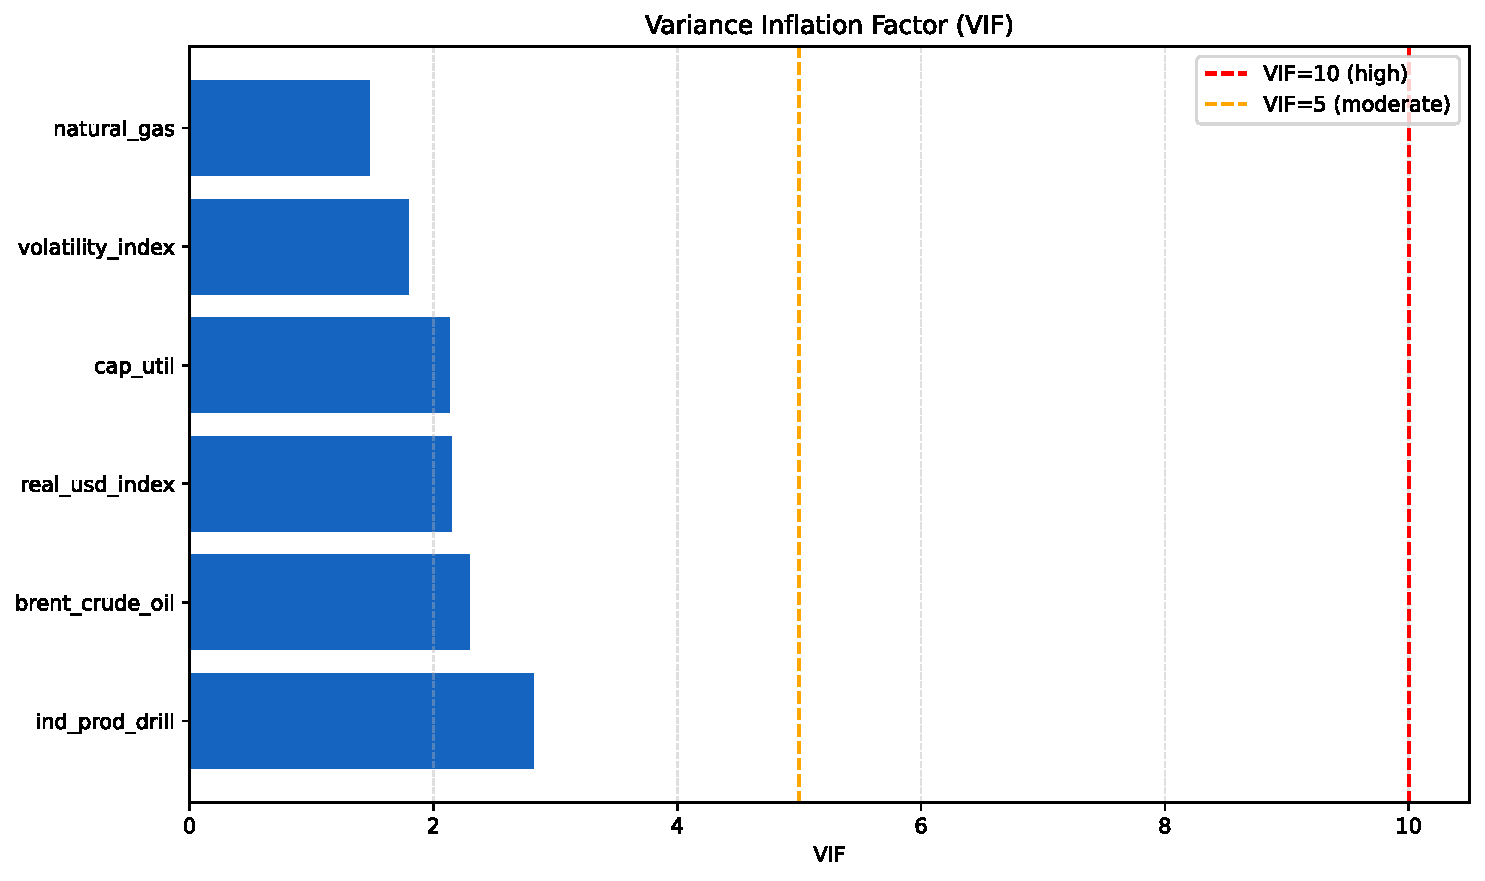
\includegraphics[width=0.88\linewidth]{vif_oil_macro_monthly_24_1_32.pdf}
\caption{Variance inflation factor (VIF) table after pruning for the WTI monthly multivariate run with $w=24, h=1, b=32$. All retained regressors satisfy $\mathrm{VIF} \le 10$, confirming that multicollinearity has been adequately controlled.}\label{fig:vif}
\end{figure}

\begin{figure}[H]
\centering
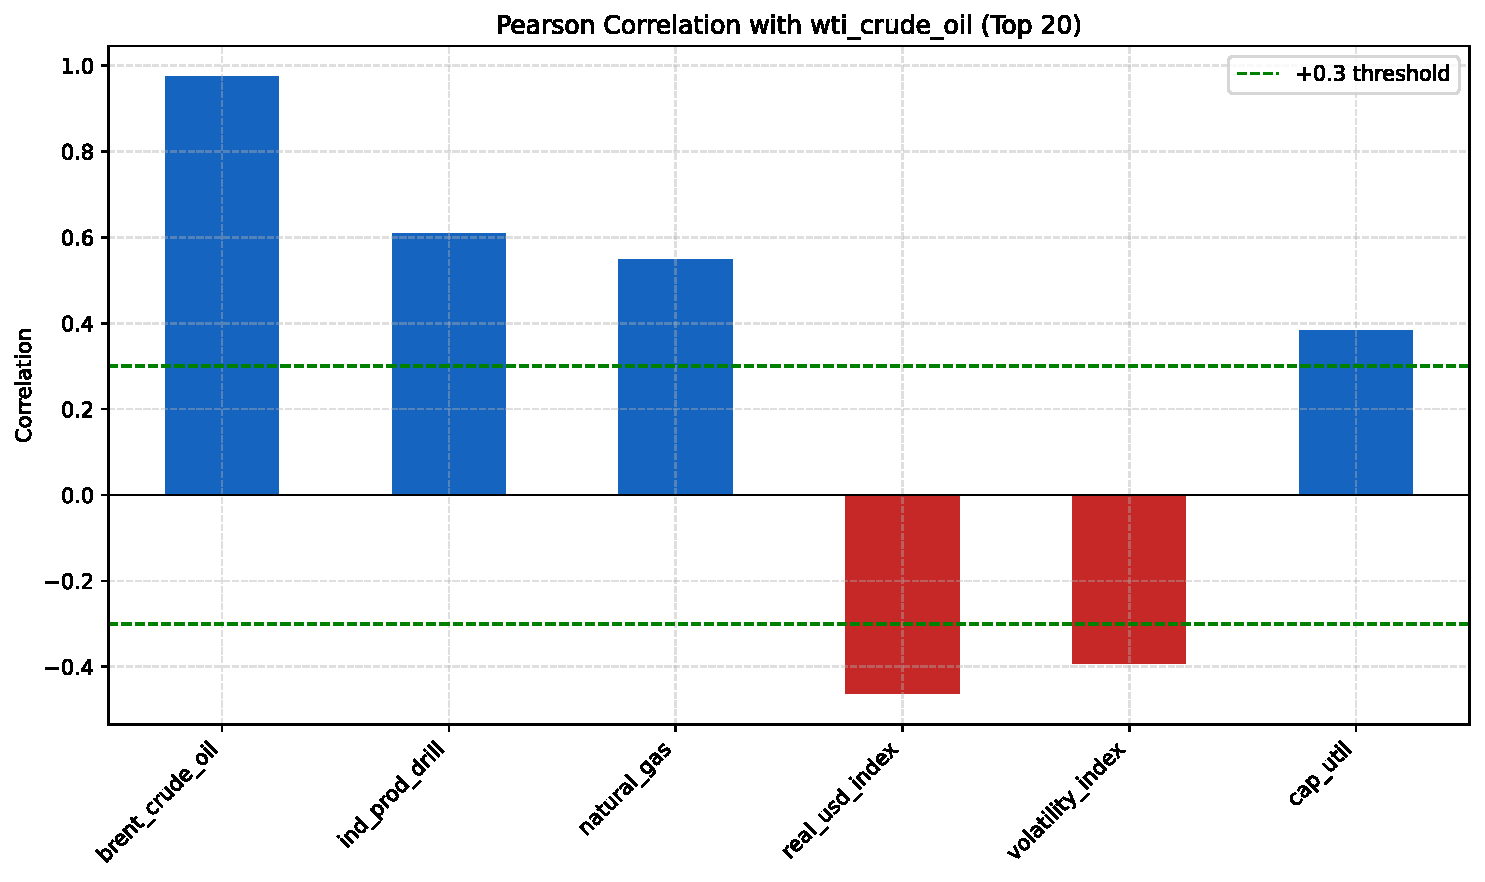
\includegraphics[width=0.95\linewidth]{pearson_oil_macro_monthly_24_1_32.pdf}
\caption{Pearson correlation matrix of the retained macro regressors for the WTI monthly multivariate run ($w=24, h=1, b=32$). The matrix reveals the pairwise linear relationship structure among the retained predictors after multicollinearity pruning.}\label{fig:pearson}
\end{figure}

\subsection{Evaluation Metrics}\label{sec:metrics}

All completed experiments are evaluated with five metrics reported on train, test, and backtest slices where available. For an evaluation slice of length $n$, with actual price $y_t$, forecast $\hat{y}_t$, and sample mean $\bar{y}$:

\begin{align}
\mathrm{MSE}  &= \frac{1}{n}\sum_{t=1}^{n}(y_t-\hat{y}_t)^2, &
\mathrm{RMSE} &= \sqrt{\frac{1}{n}\sum_{t=1}^{n}(y_t-\hat{y}_t)^2}, \nonumber\\
\mathrm{MAE}  &= \frac{1}{n}\sum_{t=1}^{n}|y_t-\hat{y}_t|, &
\mathrm{MAPE} &= \frac{100}{n}\sum_{t=1}^{n}\left|\frac{y_t-\hat{y}_t}{y_t}\right|, \label{eq:metrics}\\
R^2 &= 1-\frac{\sum_{t=1}^{n}(y_t-\hat{y}_t)^2}{\sum_{t=1}^{n}(y_t-\bar{y})^2}. \nonumber
\end{align}

RMSE and MAE are expressed in the same units as the target price and are the primary accuracy indicators. MAPE provides a unit-free relative view across commodities, but becomes unstable when actual prices are small. $R^2$ on short held-out windows must be interpreted carefully: negative values can occur when the test slice has low variance, not necessarily when the forecast is visually useless.

\subsection{System Architecture}

Figure~\ref{fig:arch} summarises the end-to-end project architecture, from public data sources through data preparation, model families, evaluation, and stored artefacts.

\begin{figure}[H]
\centering
\resizebox{\linewidth}{!}{%
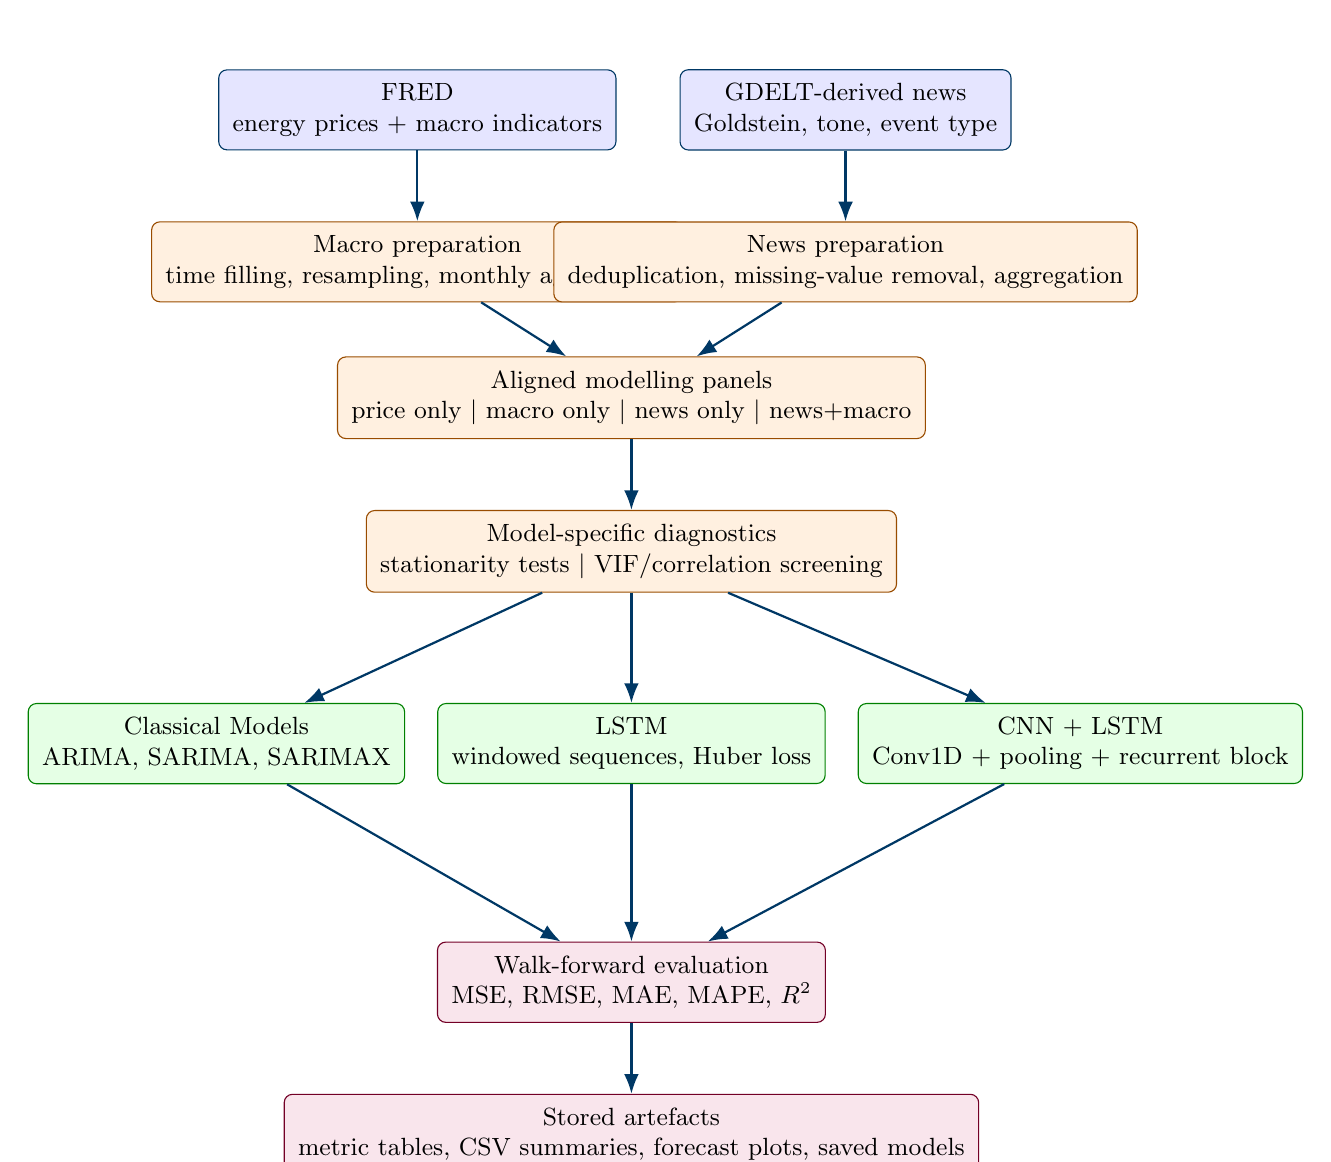
\begin{tikzpicture}[
  font=\small,
  node distance=9mm and 8mm,
  box/.style={draw, rounded corners=3pt, align=center, inner sep=5pt, minimum height=10mm},
  data/.style={box, fill=blue!10, draw=gwublue},
  prep/.style={box, fill=orange!12, draw=orange!60!black},
  model/.style={box, fill=green!10, draw=green!50!black},
  eval/.style={box, fill=purple!10, draw=purple!60!black},
  arrow/.style={-{Latex[length=2.5mm]}, thick, color=gwublue}
]
\node[data] (fred) {FRED\\energy prices + macro indicators};
\node[data, right=of fred] (gdelt) {GDELT-derived news\\Goldstein, tone, event type};
\node[prep, below=of fred] (macroprep) {Macro preparation\\time filling, resampling, monthly aggregation};
\node[prep, below=of gdelt] (newsprep) {News preparation\\deduplication, missing-value removal, aggregation};
\node[prep, below=12mm of $(macroprep)!0.5!(newsprep)$] (merge) {Aligned modelling panels\\price only $|$ macro only $|$ news only $|$ news+macro};
\node[prep, below=of merge] (diag) {Model-specific diagnostics\\stationarity tests $|$ VIF/correlation screening};
\node[model, below left=14mm and -5mm of diag] (classic) {Classical Models\\ARIMA, SARIMA, SARIMAX};
\node[model, below=14mm of diag] (lstm) {LSTM\\windowed sequences, Huber loss};
\node[model, below right=14mm and -5mm of diag] (cnnlstm) {CNN + LSTM\\Conv1D + pooling + recurrent block};
\node[eval, below=20mm of lstm] (evalnode) {Walk-forward evaluation\\MSE, RMSE, MAE, MAPE, $R^2$};
\node[eval, below=of evalnode] (artifacts) {Stored artefacts\\metric tables, CSV summaries, forecast plots, saved models};
\draw[arrow] (fred) -- (macroprep);
\draw[arrow] (gdelt) -- (newsprep);
\draw[arrow] (macroprep) -- (merge);
\draw[arrow] (newsprep) -- (merge);
\draw[arrow] (merge) -- (diag);
\draw[arrow] (diag) -- (classic);
\draw[arrow] (diag) -- (lstm);
\draw[arrow] (diag) -- (cnnlstm);
\draw[arrow] (classic) -- (evalnode);
\draw[arrow] (lstm) -- (evalnode);
\draw[arrow] (cnnlstm) -- (evalnode);
\draw[arrow] (evalnode) -- (artifacts);
\end{tikzpicture}}
\caption{End-to-end project architecture. Public data from FRED and GDELT flows through aligned modelling panels, commodity-specific diagnostics, three model families, and a walk-forward evaluation protocol to stored artefacts in the project repository.}\label{fig:arch}
\end{figure}

%% ============================================================
\section{Classical Time-Series Models}\label{sec:classical}
%% ============================================================

The classical time-series stage includes price-only univariate baselines and multivariate models with exogenous regressors. Stationarity diagnostics are applied within this stage because differencing and order selection are specific to these models.

\subsection{Stationarity Testing}

Each relevant series is subjected to the Augmented Dickey-Fuller (ADF) test~\citep{dickey1979distribution} and the Kwiatkowski-Phillips-Schmidt-Shin (KPSS) test~\citep{kwiatkowski1992testing}. The two tests are complementary: ADF tests the null of a unit root, while KPSS tests the null of stationarity. When the tests indicate non-stationarity, first differencing is applied and both tests are repeated until a stationary transformed series is confirmed. Table~\ref{tab:stationarity} shows the representative diagnostic for the differenced monthly WTI series.

\begin{table}[H]
\centering
\caption{Stationarity diagnostic for the first-differenced monthly WTI crude oil series. Both tests confirm stationarity after one round of differencing.}\label{tab:stationarity}
\small
\begin{tabular}{@{}lrrl@{}}
\toprule
\textbf{Test} & \textbf{Statistic} & \textbf{$p$-value} & \textbf{Verdict}\\
\midrule
ADF  & $-10.2774$ & $0.0000$ & Stationary \\
KPSS & $0.0355$   & $0.1000$ & Stationary \\
\bottomrule
\end{tabular}
\end{table}

\subsection{Order Selection}

Autocorrelation (ACF) and partial autocorrelation (PACF) diagnostics are used to nominate autoregressive and moving-average orders. Candidate orders are evaluated with the Akaike Information Criterion (AIC), Bayesian Information Criterion (BIC), and Hannan-Quinn Information Criterion (HQIC)~\citep{akaike1974new}. Only orders corresponding to completed stored outputs are reported.

\subsection{Seasonal Decomposition}

Monthly series are decomposed into trend, seasonal, and residual components using additive seasonal decomposition with seasonal period $s = 12$. Figure~\ref{fig:decomp} shows the decomposition panel for the WTI monthly series, which informs the seasonal order selection.

\begin{figure}[H]
\centering
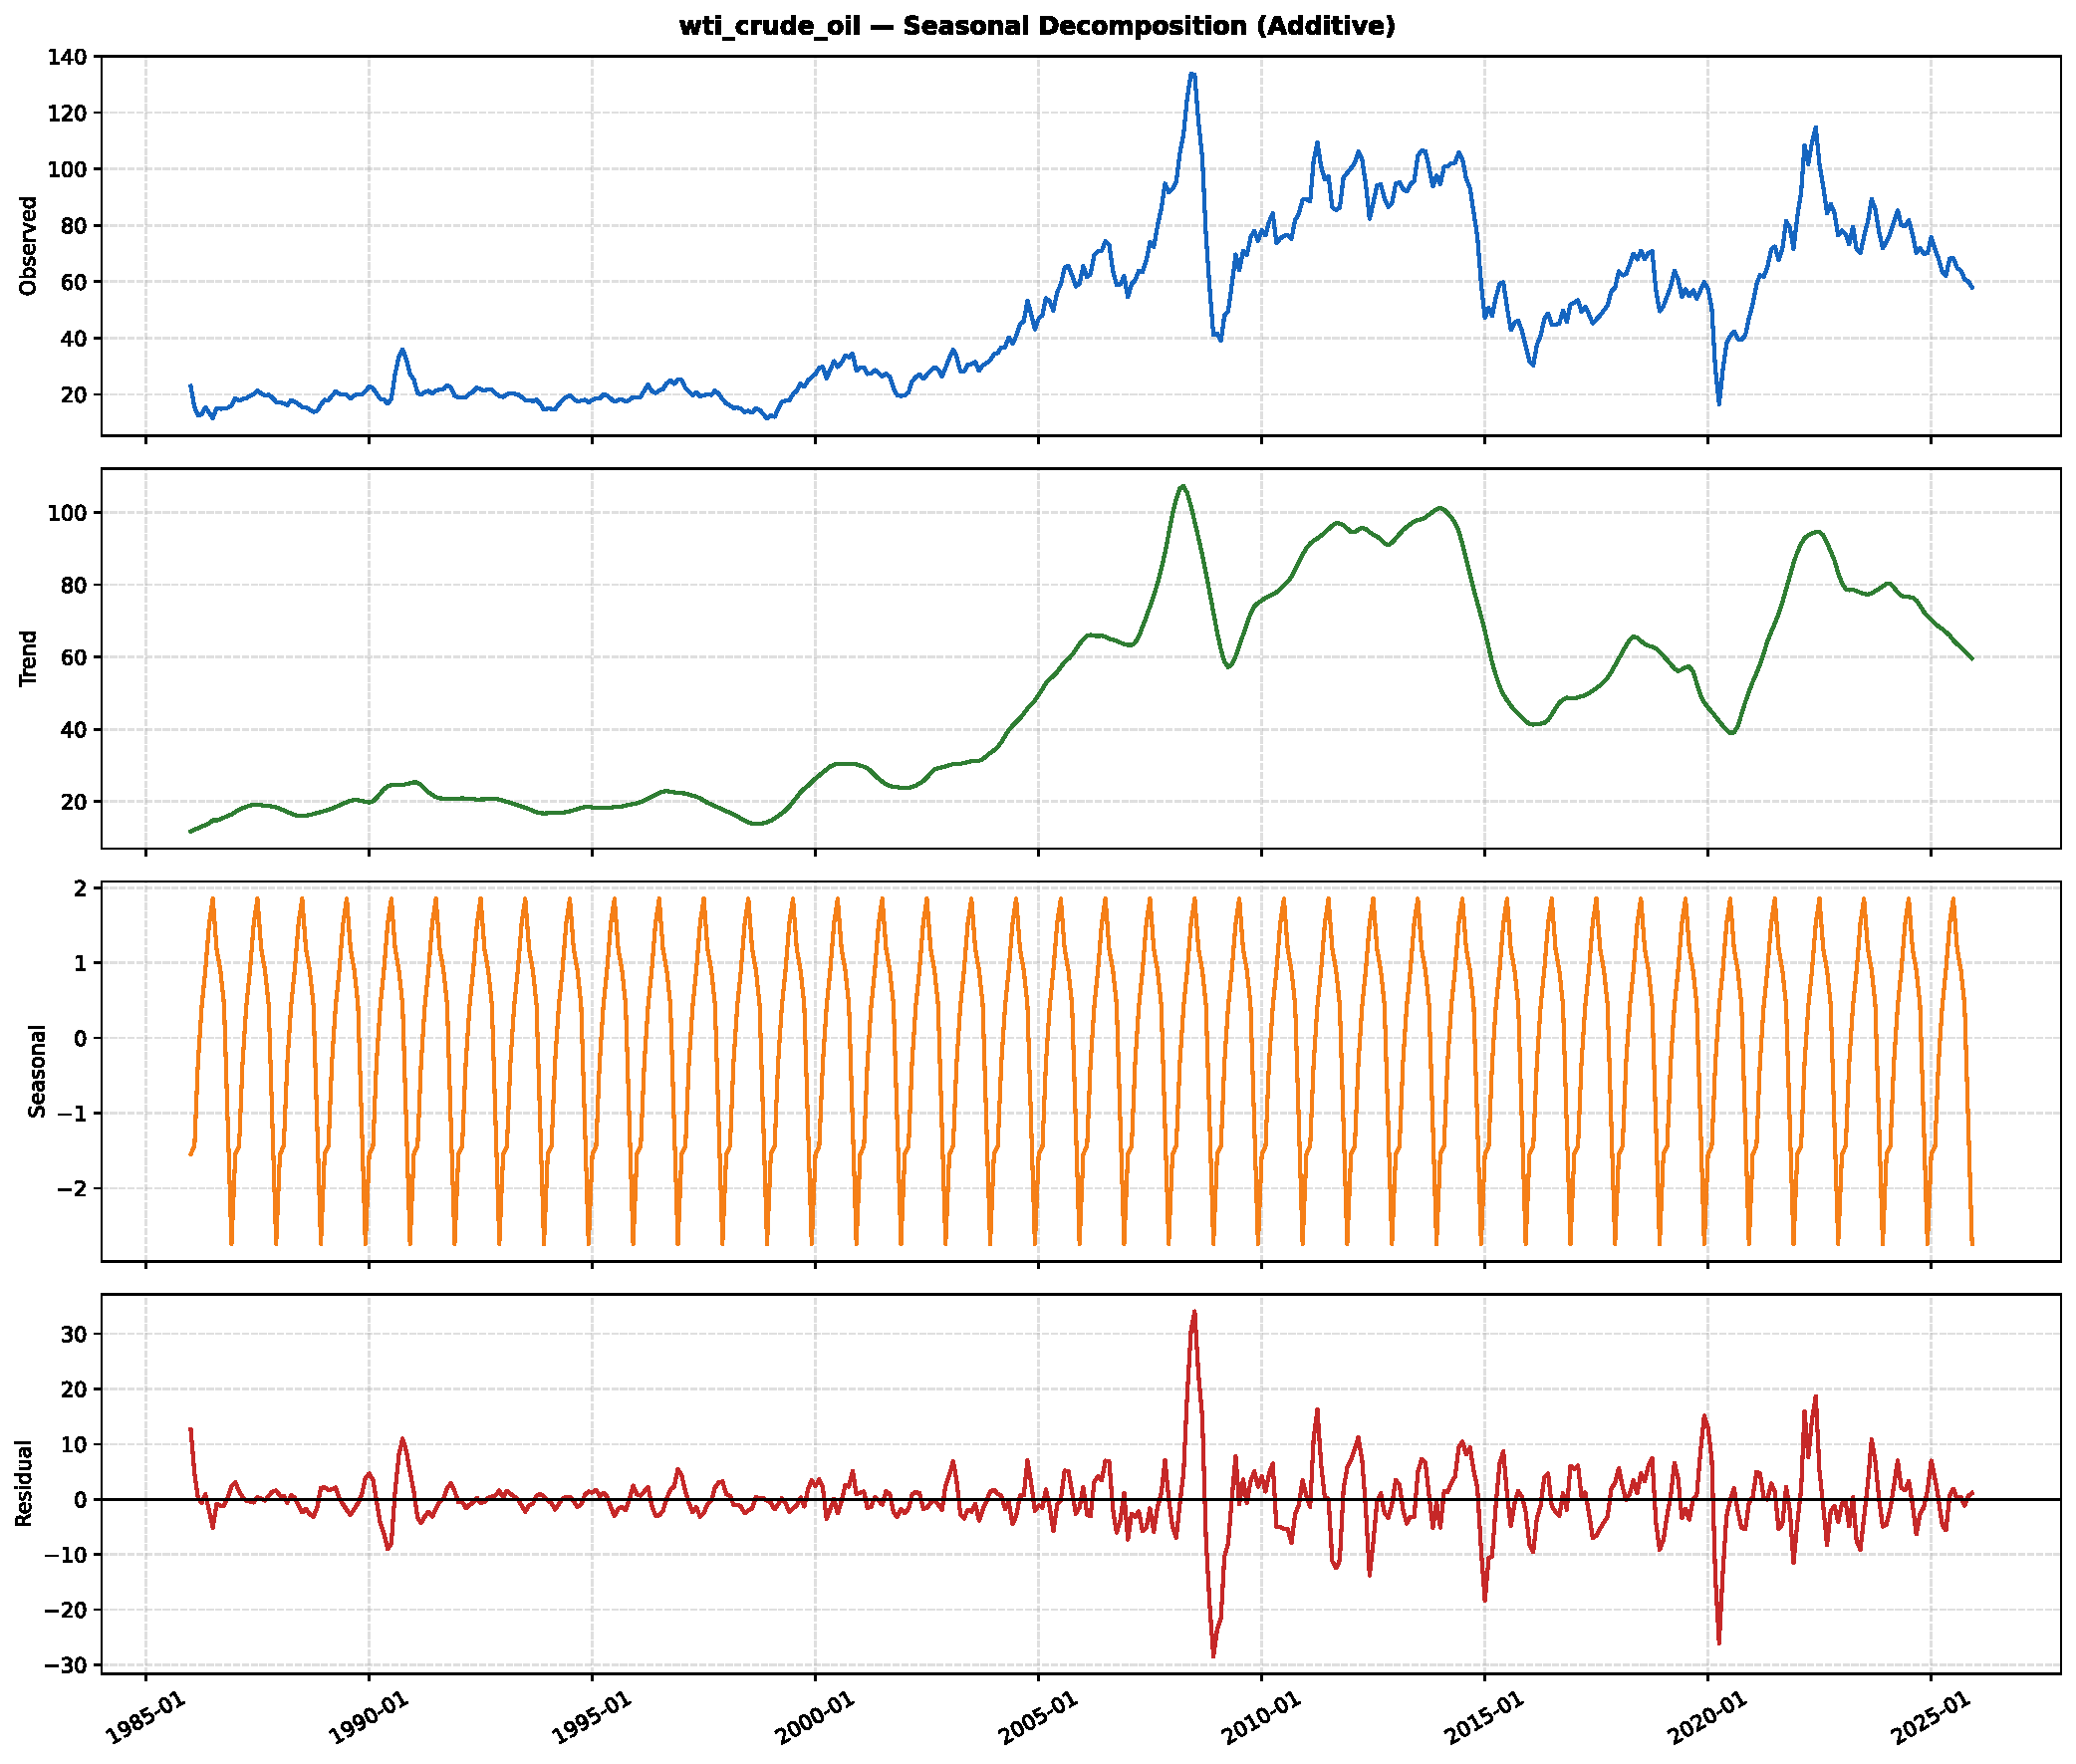
\includegraphics[width=0.95\linewidth]{oil_sarima_monthly_decomposition.pdf}
\caption{Additive seasonal decomposition of the monthly WTI crude oil series. The four panels display the original series, the trend component, the seasonal component with period $s=12$, and the residual noise.}\label{fig:decomp}
\end{figure}

\subsection{ARIMA — Autoregressive Integrated Moving Average}

The ARIMA model is used for non-seasonal endogenous dynamics. Let $B$ denote the backshift operator, $\Delta^d = (1-B)^d$ the non-seasonal differencing operator, and $\varepsilon_t$ a white-noise innovation. The ARIMA formulation is:

\begin{equation}
\phi(B)\Delta^d y_t = c + \theta(B)\varepsilon_t,
\label{eq:arima}
\end{equation}

where $\phi(B) = 1 - \phi_1 B - \cdots - \phi_p B^p$ and $\theta(B) = 1 + \theta_1 B + \cdots + \theta_q B^q$, with non-seasonal orders $(p, d, q)$.

\subsection{SARIMA — Seasonal ARIMA}

For seasonal price-only baselines, SARIMA extends ARIMA by adding seasonal autoregressive and moving-average polynomials $\Phi(B^s)$ and $\Theta(B^s)$ with seasonal period $s$:

\begin{equation}
\Phi(B^s)\phi(B)(1-B)^d(1-B^s)^D y_t
= c + \Theta(B^s)\theta(B)\varepsilon_t.
\label{eq:sarima}
\end{equation}

The seasonal orders are $(P, D, Q, s)$. For monthly experiments, $s = 12$. For daily experiments, the seasonal period is selected from stored daily diagnostic outputs.

\subsection{SARIMAX — Seasonal ARIMA with Exogenous Regressors}

SARIMAX extends the classical framework by adding an exogenous regressor matrix $\mathbf{x}_t$ with coefficient vector $\boldsymbol{\beta}$. This formulation is used for macro-only and news-plus-macro multivariate classical experiments:

\begin{equation}
\Phi(B^s)\phi(B)(1-B)^d(1-B^s)^D y_t
= c + \boldsymbol{\beta}^{\top}\mathbf{x}_t + \Theta(B^s)\theta(B)\varepsilon_t.
\label{eq:sarimax}
\end{equation}

%% ============================================================
\section{Neural Network Models}\label{sec:neural}
%% ============================================================

\subsection{LSTM — Long Short-Term Memory}

LSTM networks~\citep{hochreiter1997long,gers2000learning} address the vanishing gradient problem of standard recurrent networks through a gating mechanism. For an input sequence $\mathbf{x}_t$, the LSTM cell updates four gates:

\begin{align}
\mathbf{i}_t &= \sigma(W_i\mathbf{x}_t + U_i\mathbf{h}_{t-1} + \mathbf{b}_i), &
\mathbf{f}_t &= \sigma(W_f\mathbf{x}_t + U_f\mathbf{h}_{t-1} + \mathbf{b}_f), \nonumber\\
\tilde{\mathbf{c}}_t &= \tanh(W_c\mathbf{x}_t + U_c\mathbf{h}_{t-1} + \mathbf{b}_c), &
\mathbf{o}_t &= \sigma(W_o\mathbf{x}_t + U_o\mathbf{h}_{t-1} + \mathbf{b}_o), \label{eq:lstm-gates}\\
\mathbf{c}_t &= \mathbf{f}_t \odot \mathbf{c}_{t-1} + \mathbf{i}_t \odot \tilde{\mathbf{c}}_t, &
\mathbf{h}_t &= \mathbf{o}_t \odot \tanh(\mathbf{c}_t). \nonumber
\end{align}

The forecast head maps the final hidden representation to the horizon-specific prediction $\hat{\mathbf{y}}_{t+1:t+h}$.

\paragraph{Architecture.} The multivariate LSTM configuration uses two stacked recurrent layers with L2 regularisation, followed by a dense layer with ReLU activation, a dropout layer, and a linear forecast head. The univariate LSTM is trained on a single-feature price sequence.

\subsection{CNN + LSTM — Convolutional Recurrent Network}

The CNN\,+\,LSTM configuration~\citep{sainath2015convolutional,lecun1998gradient} prepends a one-dimensional convolution and max-pooling step before the recurrent block. The convolution transforms a windowed feature sequence into local temporal features:

\begin{equation}
\mathbf{z}_{t,k} = g\!\left(b_k + \sum_{j=0}^{K-1} W_{k,j}^{\top}\mathbf{x}_{t+j}\right),
\label{eq:conv1d}
\end{equation}

where $K$ is the kernel width, $k$ indexes the filter, and $g(\cdot)$ is the ReLU activation. The pooled convolutional sequence is then passed through the LSTM update in Eq.~\eqref{eq:lstm-gates}.

\paragraph{Architecture.} The CNN layer uses 64 filters with kernel size 3 and same padding. Max-pooling with pool size 2 reduces the temporal dimension. The pooled output feeds into a single LSTM layer, a dense projection, and a linear forecast head.

\subsection{Training Setup}

\begin{itemize}[leftmargin=*]
  \item \textbf{Optimiser:} Adam~\citep{kingma2015adam} with initial learning rate selected by Optuna~\citep{akiba2019optuna}.
  \item \textbf{Loss function:} Huber loss~\citep{huber1964robust} for robustness to price spikes:
  \begin{equation}
    \mathcal{L}_{\delta}(e_t) =
    \begin{cases}
      \tfrac{1}{2}e_t^2, & |e_t| \le \delta,\\
      \delta\!\left(|e_t| - \tfrac{1}{2}\delta\right), & |e_t| > \delta.
    \end{cases}
    \label{eq:huber}
  \end{equation}
  \item \textbf{Regularisation:} L2 weight decay, dropout (0.1–0.3), early stopping (patience 10) on validation Huber loss, and ReduceLROnPlateau (factor 0.5, patience 5, min\_lr $10^{-6}$).
  \item \textbf{Hyperparameter tuning:} Optuna Bayesian optimisation over 30 trials for LSTM units, dropout rate, L2 regularisation coefficient, and learning rate.
  \item \textbf{Data split:} 90\% training, 10\% validation within the train block. Shuffle is disabled to preserve temporal ordering.
\end{itemize}

%% ============================================================
\section{Results and Analysis}\label{sec:results}
%% ============================================================

This section reports only completed configurations with stored metric artefacts. Every number in the tables below is traced to a CSV summary or rendered metric panel in the project repository. The discussion emphasises whether each configuration captures price fluctuations clearly and whether the forecast path is stable across the held-out slice.

\subsection{Univariate Baselines}\label{sec:res-uni}

Table~\ref{tab:uni-results} presents the selected univariate model outputs for both WTI crude oil and Henry Hub natural gas. These baselines isolate the information contained in the target series alone.

\begin{table}[H]
\centering
\caption{Selected univariate model outputs. Metrics are reported on the test slice. Configurations are included only where stored metric artefacts are available.}\label{tab:uni-results}
\small
\resizebox{\linewidth}{!}{%
\begin{tabular}{@{}lllllrrrr@{}}
\toprule
\textbf{Commodity} & \textbf{Freq.} & \textbf{Model} & \textbf{Configuration} & \textbf{RMSE} & \textbf{MAE} & \textbf{MAPE\%} & \textbf{$R^2$} \\
\midrule
Oil & M & ARIMA  & $(0,1,1)$                             & 6.832  & 6.343  & 10.494 & $-6.242$  \\
Oil & D & SARIMA & $(1,1,0)\!\times\!(0,1,0,12)$          & 1.210  & 1.081  &  1.868 & $-1.955$  \\
Oil & M & LSTM   & $(5,1,32)$                             & 16.176 & 10.683 & 18.055 & $-39.589$ \\
CNG & M & ARIMA  & $(0,1,0)$                             & 0.541  & 0.447  & 12.256 & $-0.139$  \\
CNG & M & SARIMA & $(0,1,0)\!\times\!(0,1,0,12)$          & 0.376  & 0.310  &  9.339 & $+0.449$  \\
CNG & M & LSTM   & $(5,1,32)$                             & 0.554  & 0.497  & 14.721 & $-0.194$  \\
\bottomrule
\end{tabular}}
\end{table}

\paragraph{WTI crude oil univariate results.} The daily SARIMA achieves the lowest RMSE at 1.210 and MAPE at 1.868\%, showing that short-horizon daily dynamics are well captured by seasonal differencing on the own price path. The monthly ARIMA provides a usable medium-frequency baseline (RMSE 6.832, MAPE 10.494\%), while the monthly LSTM underperforms (RMSE 16.176, MAPE 18.055\%) with a strongly negative $R^2$, suggesting that a short price-only window of 5 steps is insufficient for neural learning in the monthly oil setting.

\paragraph{Henry Hub natural gas univariate results.} The monthly SARIMA is the strongest univariate configuration, achieving RMSE 0.376, MAPE 9.339\%, and the only positive $R^2 = +0.449$ in this group. This indicates that the seasonal structure of the natural gas series (period $s=12$) provides genuine predictive signal. Both ARIMA and LSTM produce acceptable errors in absolute terms but marginally negative $R^2$ values on the held-out slice.

Figure~\ref{fig:uni-oil-forecast} shows the two-order aggregated SARIMA forecast for WTI monthly, illustrating the visual quality of the best-performing aggregated seasonal model.

\begin{figure}[H]
\centering
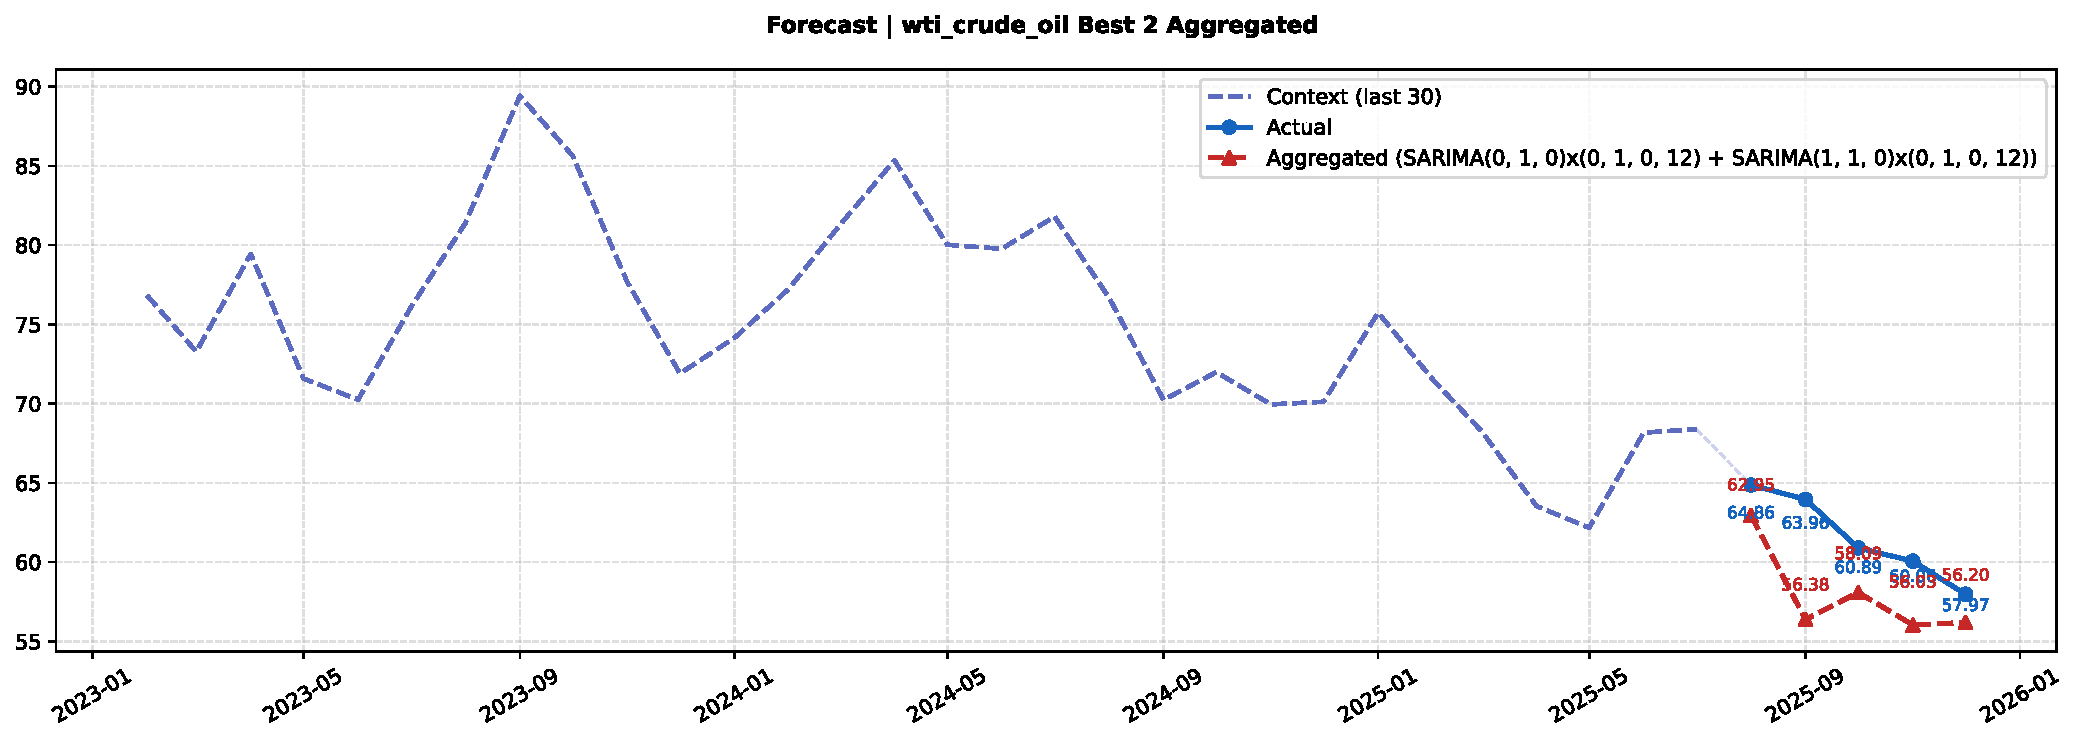
\includegraphics[width=0.88\linewidth]{oil_sarima_monthly_aggregated_forecast.pdf}
\caption{Two-order aggregated SARIMA forecast on the WTI monthly test block versus the actual price path. The forecast tracks the general direction of movement, though it lags the magnitude of sharp price movements.}\label{fig:uni-oil-forecast}
\end{figure}

\subsection{Multivariate Models — WTI Crude Oil}\label{sec:res-multi-oil}

Table~\ref{tab:oil-multi} reports the selected multivariate outputs for WTI crude oil across the macro-only, news-only, and fused news-plus-macro input settings.

\begin{table}[H]
\centering
\caption{Selected multivariate outputs for WTI crude oil. The news-plus-macro LSTM (24,5,32) achieves the lowest monthly RMSE of 2.921 at a five-step horizon.}\label{tab:oil-multi}
\small
\resizebox{\linewidth}{!}{%
\begin{tabular}{@{}lllllrrrr@{}}
\toprule
\textbf{Input Set} & \textbf{Freq.} & \textbf{Model} & \textbf{Configuration} & \textbf{RMSE} & \textbf{MAE} & \textbf{MAPE\%} & \textbf{$R^2$} \\
\midrule
Macro only     & M & CNN + LSTM & $(36,1,32)$                          & 8.342 & 7.008 & 11.763 & $-13.837$ \\
News only      & M & CNN + LSTM & $(24,5,32)$                          & 6.648 & 4.605 &  7.803 & $-8.711$  \\
News + Macro   & D & SARIMAX    & $(0,1,1)\!\times\!(0,1,0,9)$         & 1.235 & 1.109 &  1.681 & $-2.166$  \\
News + Macro   & M & LSTM       & $(24,5,32)$                          & 2.921 & 2.378 &  4.011 & $-0.875$  \\
News + Macro   & M & CNN + LSTM & $(36,5,32)$                          & 5.730 & 5.060 &  8.234 & $-6.214$  \\
\bottomrule
\end{tabular}}
\end{table}

\paragraph{Key observations.} The news-plus-macro LSTM (24,5,32) produces the lowest monthly RMSE at 2.921 and the lowest monthly MAPE at 4.011\%, a substantial improvement over both the macro-only and news-only configurations. The daily SARIMAX captures short-horizon fluctuations with RMSE 1.235 and MAPE 1.681\%, competitive with the univariate daily SARIMA. The macro-only CNN\,+\,LSTM (36,1,32) has the highest monthly RMSE at 8.342, indicating that the macro block alone at a long one-step window does not provide consistent improvement over the univariate benchmark for WTI.

Figure~\ref{fig:oil-selected} shows the forecast path and learning curves for the best-performing configuration — the news-plus-macro LSTM (24,5,32).

\begin{figure}[H]
\centering
\begin{subfigure}[b]{0.49\textwidth}
  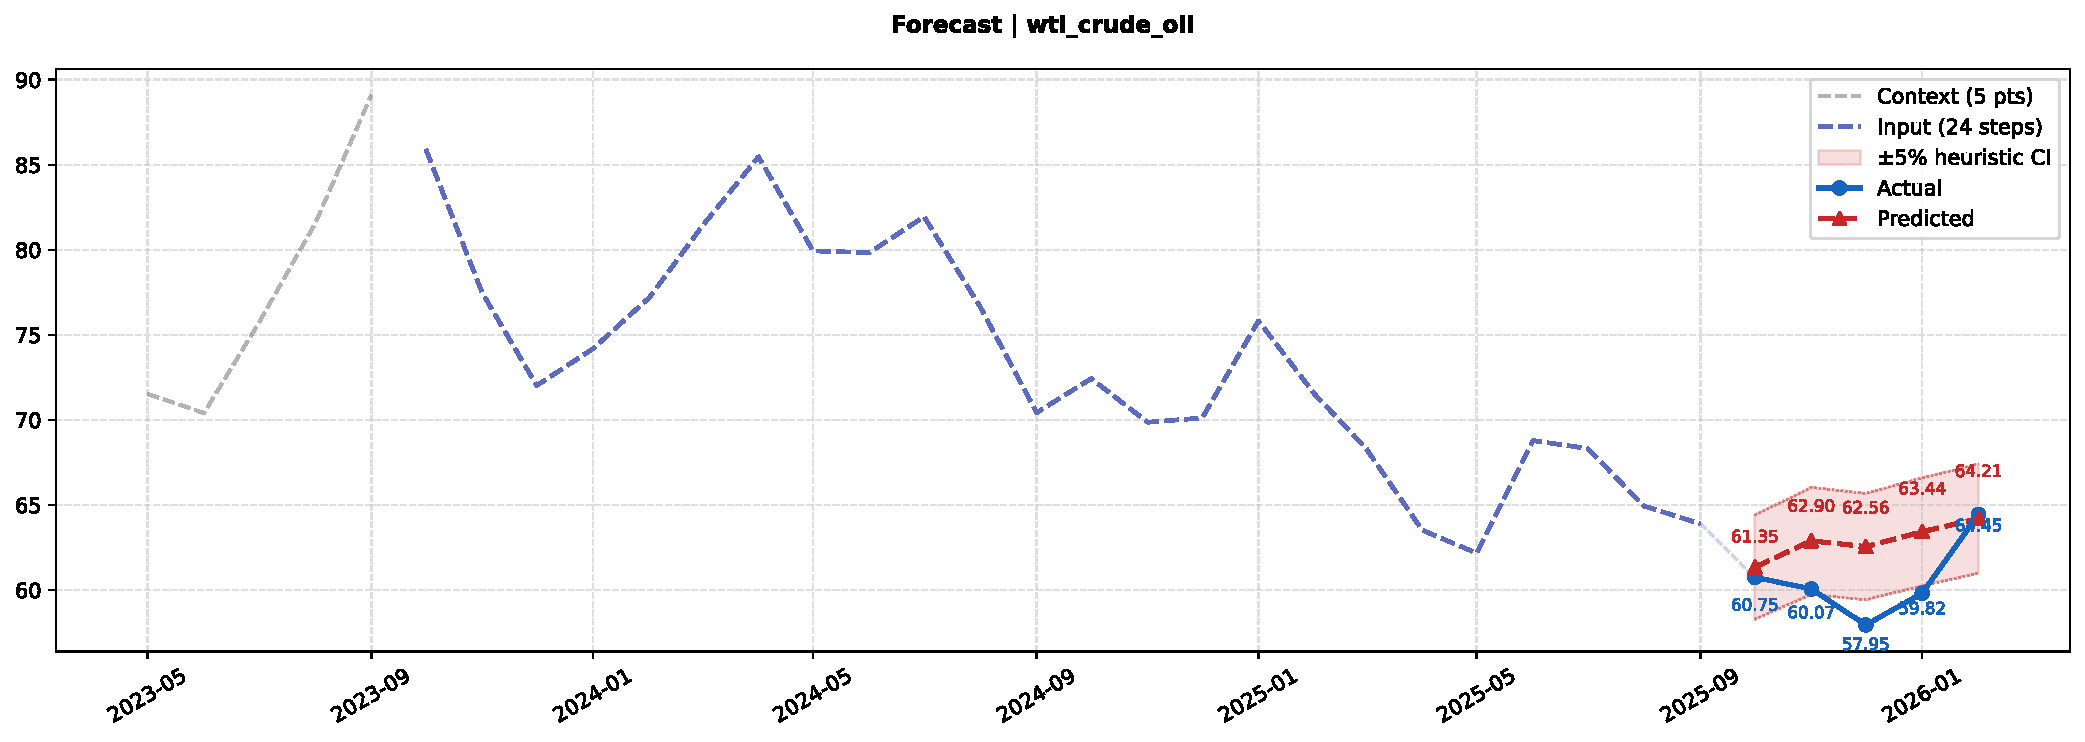
\includegraphics[width=\linewidth]{oil_news_macro_lstm_24_5_32_forecast.pdf}
  \caption{Five-step ahead forecast vs.\ actual WTI price on the held-out test block.}
\end{subfigure}\hfill
\begin{subfigure}[b]{0.49\textwidth}
  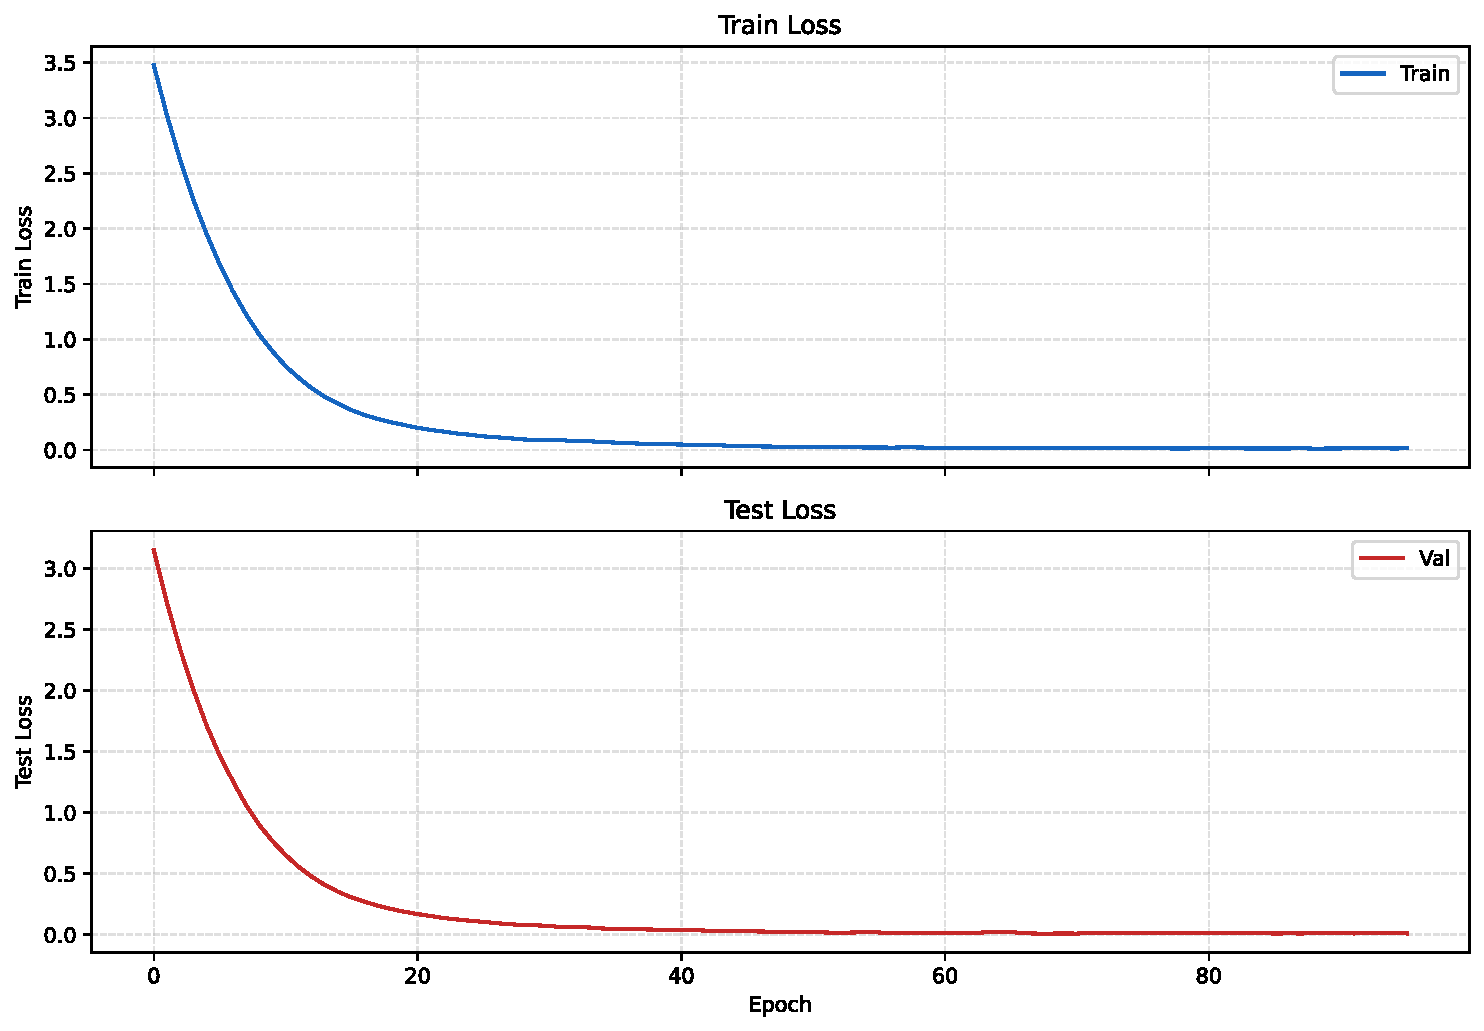
\includegraphics[width=\linewidth]{oil_news_macro_lstm_24_5_32_loss.pdf}
  \caption{Training and validation Huber loss curves across training epochs.}
\end{subfigure}
\caption{WTI monthly LSTM trained on news-plus-macro inputs, configuration $(w=24, h=5, b=32)$. The forecast panel shows a coherent five-step trajectory, and the loss curves indicate stable convergence without severe overfitting.}\label{fig:oil-selected}
\end{figure}

\subsection{Multivariate Models — Henry Hub Natural Gas}\label{sec:res-multi-cng}

Table~\ref{tab:cng-multi} reports the selected multivariate outputs for Henry Hub natural gas. The news-plus-macro fused setting yields the best overall performance.

\begin{table}[H]
\centering
\caption{Selected multivariate outputs for Henry Hub natural gas. The news-plus-macro CNN\,+\,LSTM (36,5,32) achieves the best test RMSE of 1.153 with the only positive $R^2 = +0.550$.}\label{tab:cng-multi}
\small
\resizebox{\linewidth}{!}{%
\begin{tabular}{@{}lllllrrrr@{}}
\toprule
\textbf{Input Set} & \textbf{Freq.} & \textbf{Model} & \textbf{Configuration} & \textbf{RMSE} & \textbf{MAE} & \textbf{MAPE\%} & \textbf{$R^2$} \\
\midrule
Macro only   & M & LSTM       & $(36,1,32)$                    & 1.526 & 1.227 & 26.348  & $+0.215$ \\
Macro only   & M & CNN + LSTM & $(36,1,32)$                    & 1.801 & 1.313 & 25.897  & $-0.093$ \\
News only    & M & CNN + LSTM & $(36,1,32)$                    & 4.357 & 3.932 & 107.173 & $-5.412$ \\
News + Macro & M & LSTM       & $(36,5,32)$                    & 1.727 & 1.501 & 33.432  & $-0.008$ \\
News + Macro & M & CNN + LSTM & $(36,5,32)$                    & 1.153 & 0.943 & 22.204  & $+0.550$ \\
News + Macro & D & SARIMAX    & $(0,1,1)\!\times\!(0,1,0,6)$  & 0.087 & 0.080 &  2.661  & $-0.879$ \\
\bottomrule
\end{tabular}}
\end{table}

\paragraph{Key observations.} The news-plus-macro CNN\,+\,LSTM (36,5,32) is the standout performer for Henry Hub with RMSE 1.153, MAE 0.943, and $R^2 = +0.550$, the only clearly positive $R^2$ across all multivariate neural experiments. The macro-only LSTM (36,1,32) also achieves a positive $R^2 = +0.215$, suggesting that macroeconomic context provides genuine signal for natural gas at the monthly horizon.

The news-only CNN\,+\,LSTM (36,1,32) performs poorly with MAPE 107.17\%, indicating that the GDELT-derived news block alone is insufficient as a standalone signal for natural gas forecasting. The daily SARIMAX achieves a remarkably low absolute error (RMSE 0.087, MAE 0.080, MAPE 2.661\%), though the negative $R^2$ reflects sensitivity to the short-horizon test slice variance.

Figure~\ref{fig:cng-selected} shows the forecast and backtest panels for the best-performing configuration — the news-plus-macro CNN\,+\,LSTM (36,5,32).

\begin{figure}[H]
\centering
\begin{subfigure}[b]{0.49\textwidth}
  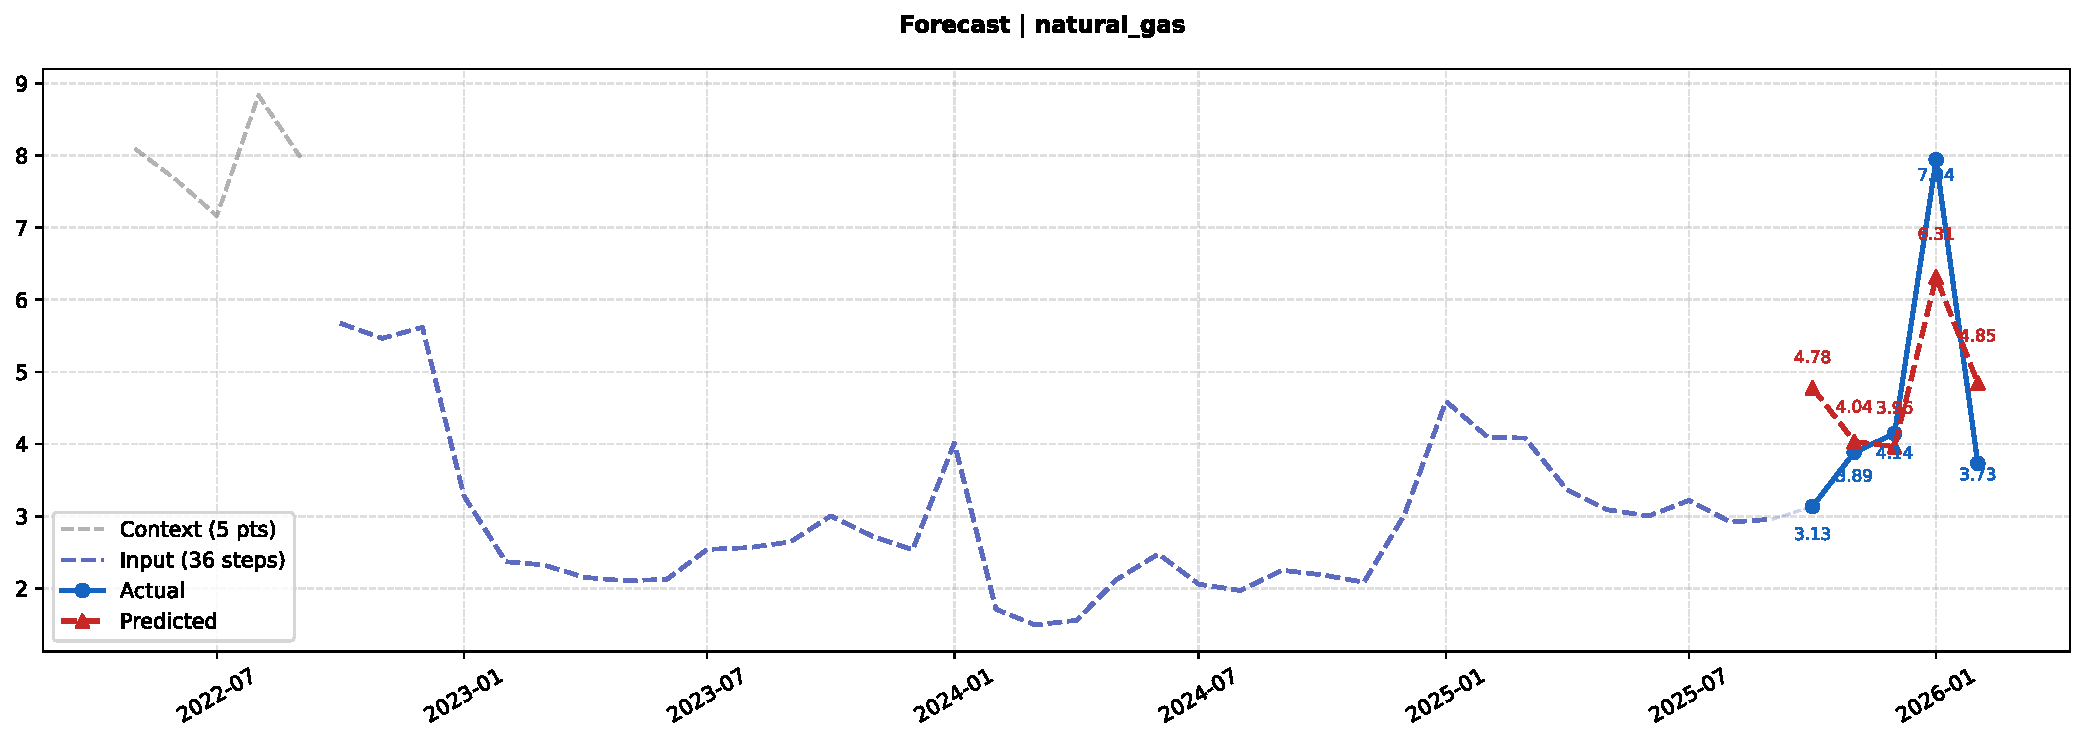
\includegraphics[width=\linewidth]{cng_news_macro_cnn_lstm_36_5_32_forecast.pdf}
  \caption{Five-step forecast vs.\ actual Henry Hub price on the test block.}
\end{subfigure}\hfill
\begin{subfigure}[b]{0.49\textwidth}
  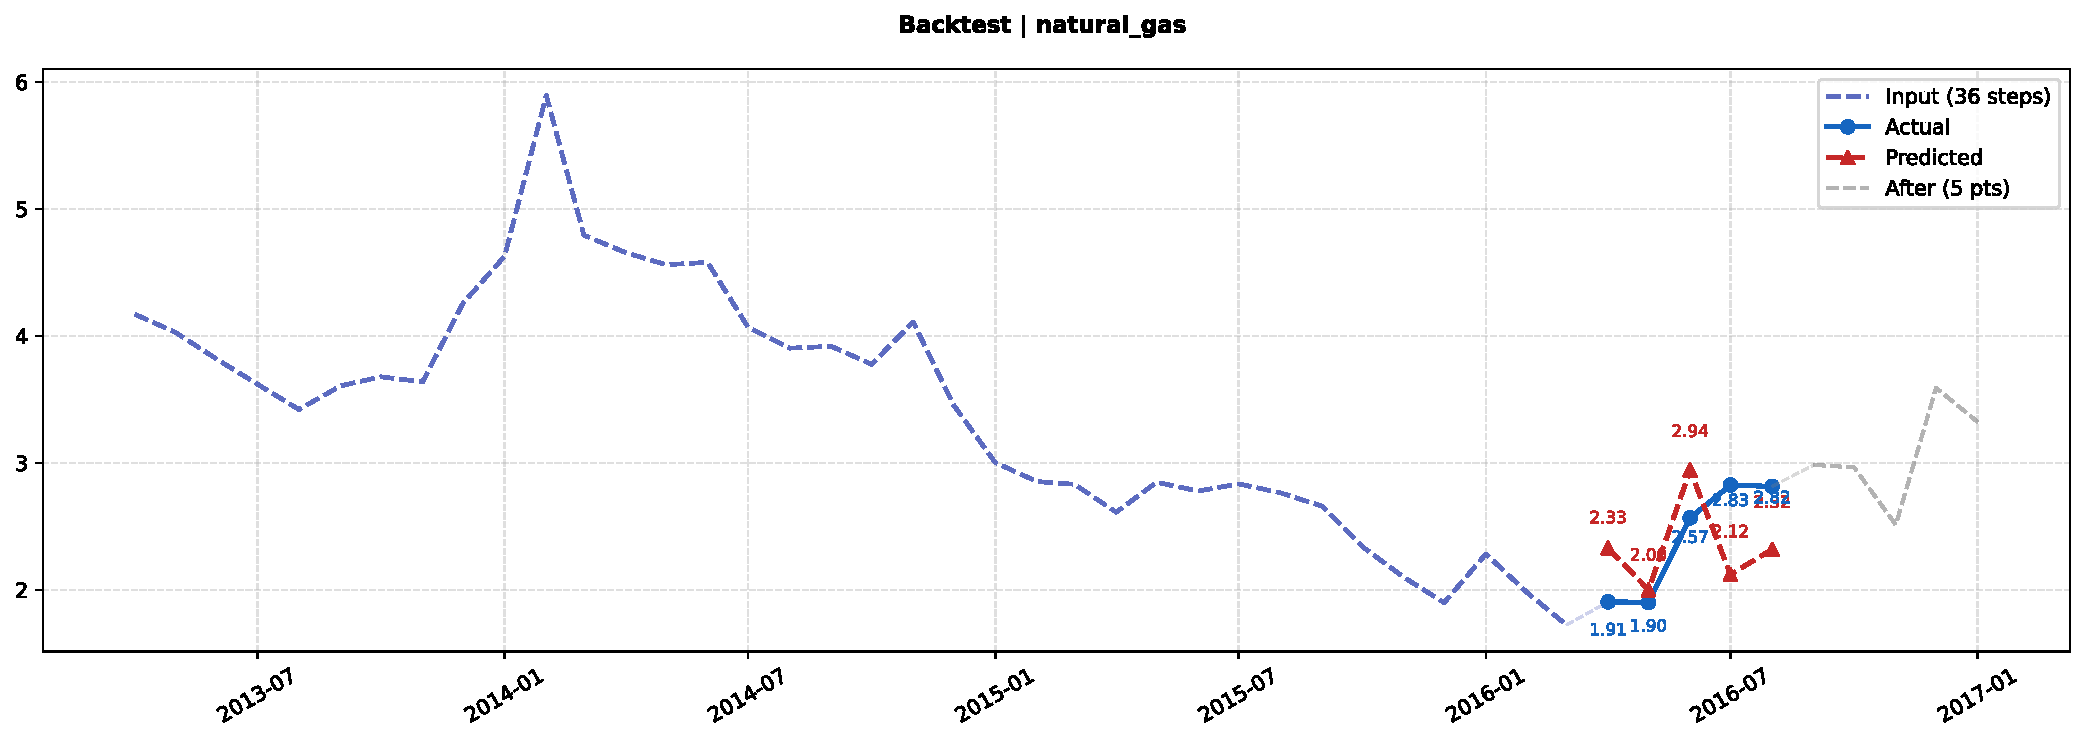
\includegraphics[width=\linewidth]{cng_news_macro_cnn_lstm_36_5_32_backtest.pdf}
  \caption{Backtest panel showing out-of-training performance on the diagnostic block.}
\end{subfigure}
\caption{Henry Hub monthly CNN\,+\,LSTM trained on news-plus-macro inputs, configuration $(w=36, h=5, b=32)$. The forecast panel shows stable monthly movement on the test horizon; the backtest panel provides an additional diagnostic view of generalisation stability outside the training window.}\label{fig:cng-selected}
\end{figure}

\subsection{Summary Comparison}

Table~\ref{tab:summary-comparison} provides a consolidated view of the best-performing configuration for each combination of commodity, frequency, and information setting, enabling direct cross-condition comparison.

\begin{table}[H]
\centering
\caption{Summary of best test-slice RMSE per condition. Each cell shows the minimum RMSE achieved and the corresponding model configuration.}\label{tab:summary-comparison}
\small
\resizebox{\linewidth}{!}{%
\begin{tabular}{@{}llllll@{}}
\toprule
\textbf{Commodity} & \textbf{Freq.} & \textbf{Price-Only} & \textbf{Macro} & \textbf{News} & \textbf{News+Macro} \\
\midrule
WTI  & Daily   & 1.210 (SARIMA) & — & — & 1.235 (SARIMAX) \\
WTI  & Monthly & 6.832 (ARIMA)  & 8.342 (CNN+LSTM) & 6.648 (CNN+LSTM) & \textbf{2.921} (LSTM) \\
CNG  & Daily   & — & — & — & \textbf{0.087} (SARIMAX) \\
CNG  & Monthly & 0.376 (SARIMA) & 1.526 (LSTM) & 4.357 (CNN+LSTM) & \textbf{1.153} (CNN+LSTM) \\
\bottomrule
\end{tabular}}
\end{table}

%% ============================================================
\section{Discussion}\label{sec:discussion}
%% ============================================================

\subsection{Value of News-Plus-Macro Fusion}

The GDELT-derived news block contributes most clearly when fused with macroeconomic variables rather than used as a standalone signal. On WTI monthly, the news-plus-macro LSTM (24,5) produces a coherent five-step path and substantially reduces RMSE from 6.832 (univariate baseline) to 2.921. On Henry Hub monthly, the news-plus-macro CNN\,+\,LSTM (36,5) follows the direction of the held-out movement with $R^2 = +0.550$, the strongest variance-explained result across all experiments. On WTI daily, the news-plus-macro SARIMAX captures short-horizon fluctuations with MAPE 1.681\%.

A plausible interpretation is that the news block functions as a slow-moving regime variable. Its informational content is easier to observe at the monthly horizon, where persistent direction of policy and macroeconomic narrative reporting can be aggregated into a meaningful exogenous signal. At daily frequency, the same block is more sensitive to short-horizon noise, and stable behaviour appears only when the model structure and differencing procedure dampen that noise.

\subsection{Commodity Differences}

The commodity difference is structurally important. WTI crude oil is heavily exposed to broad macro-financial and geopolitical narratives, so a news-plus-macro representation has a clearer interpretation in the monthly WTI experiments. Henry Hub natural gas, by contrast, often responds to regional demand, storage cycles, and weather-related pressures that are not fully captured by the current feature set. This accounts for the higher MAPE values observed in the Henry Hub neural results (22–33\%) even when the $R^2$ is positive.

\subsection{Classical vs.\ Neural Behaviour}

The classical outputs remain informative because they require relatively few parameters and respond directly to stationarity and seasonal structure. The neural outputs become more useful when longer windows and fused exogenous inputs are available, especially in monthly settings where the signal-to-noise ratio is higher than at the daily frequency. This pattern is consistent with the training-data constraint: recurrent models require enough contiguous sequences to learn stable dynamics, while classical models can remain steady under shorter samples.

The distinction is methodological rather than philosophical. Classical models offer transparency through differencing, order selection, and explicit exogenous coefficients. Neural models offer flexibility through nonlinear sequence transformations, but the same flexibility can amplify noise when the training sample is short. The most interpretable neural outputs are therefore configurations whose forecast plots show smooth movement and whose training curves do not separate sharply between training and validation loss.

\subsection{Hyperparameter Sensitivity}

Across the neural experiments, test RMSE is non-monotonic in the input window. Longer windows provide more historical context, but also reduce the number of admissible training sequences. The stored outputs suggest a practical trade-off: windows such as $(24,5)$ and $(36,5)$ can capture multi-step movement, while very long windows may compress the effective training set too severely for stable generalisation. The WTI monthly news-plus-macro LSTM illustrates this: its $(24,5)$ configuration produces a coherent five-step trajectory, suggesting that direct multi-step forecasting can act as a regularising constraint.

%% ============================================================
\section{Limitations}\label{sec:limits}
%% ============================================================

This study is subject to the following limitations, which should be considered when interpreting the results.

\paragraph{Alignment and aggregation smoothing.} The public macroeconomic and news-derived datasets have different native frequencies and reporting calendars. Alignment and aggregation may smooth or delay parts of the signal, particularly for monthly GDELT aggregates.

\paragraph{Finite test windows.} The test windows are finite and should be interpreted as held-out point estimates rather than full uncertainty intervals. The short length of some test slices makes $R^2$ particularly sensitive to variance.

\paragraph{External shocks not fully captured.} The models remain sensitive to external events — geopolitical shocks, weather disruptions, policy changes, and sudden demand shifts — that may not be fully represented by the available features. No model in this framework can be expected to anticipate truly unprecedented events.

\paragraph{Breadth of completed experiments.} Only configurations with complete stored metric artefacts are included in the tables. This protects reproducibility and factual correctness but limits the breadth of the comparison relative to all attempted configurations.

\paragraph{Event-level news representation.} The available news representation is event-level and numeric. It does not preserve full article text, source identity, or topic-level nuance beyond the retained GDELT fields. The design is therefore appropriate for a reproducible tabular forecasting study, but cannot answer finer questions about which individual stories or narrative themes drove particular forecast movements.

%% ============================================================
\section{Future Work}\label{sec:future-work}
%% ============================================================

Future work can extend this project in four directions.

\paragraph{Feature engineering.} Adding lagged macro variables, rolling volatility summaries, shock indicators, inventory release dummies, and richer transformations of the news features (such as topic-level sentiment or entity-filtered event counts) may capture causal mechanisms more precisely.

\paragraph{Advanced architectures.} Temporal Convolutional Networks (TCN), Transformer-based sequence models, and attention mechanisms with interpretable alignment maps can be evaluated under the same walk-forward protocol once sufficient training data and stored artefacts are available.

\paragraph{Real-time pipeline.} The data and modelling pipeline can be adapted for real-time forecasting so that new FRED releases and GDELT events automatically update the feature panel and trigger re-evaluation without manual intervention.

\paragraph{Additional external data.} Weather variables, shipping and freight indicators, weekly EIA storage reports, satellite-derived oil-storage estimates, and geopolitical-event datasets from alternative providers can be integrated to capture drivers that are not fully represented in the current input blocks.

%% ============================================================
\section{Conclusion}\label{sec:conclusion}
%% ============================================================

This report presents a reproducible, systematic comparison of univariate and multivariate forecasting approaches for WTI crude oil and Henry Hub natural gas prices at both daily and monthly frequencies. The experimental framework evaluates three classical model families (ARIMA, SARIMA, SARIMAX) and two deep-learning architectures (LSTM, CNN\,+\,LSTM) across four information settings: price-only, macro-only, news-only, and fused news-plus-macro.

The results establish three principal findings:

\begin{enumerate}[leftmargin=*]
  \item \textbf{Fused information is superior.} The news-plus-macro input setting consistently delivers the strongest neural results on both commodities: RMSE 2.921 for WTI monthly LSTM (24,5) and RMSE 1.153 ($R^2 = +0.550$) for Henry Hub monthly CNN\,+\,LSTM (36,5). The news block alone is insufficient as a standalone signal.

  \item \textbf{Forecasting behaviour is frequency- and commodity-specific.} Daily classical models achieve the lowest absolute errors through differencing and short-horizon sensitivity. Monthly experiments benefit more from exogenous fusion, especially for WTI. Henry Hub natural gas is harder to forecast with current macro and news signals alone, reflecting its regional supply-demand dynamics.

  \item \textbf{Classical models remain competitive.} Daily SARIMA and SARIMAX achieve MAPE values below 2.7\% on both commodities. For shorter samples and at daily frequency, classical models with explicit seasonal structure often match or outperform deep learning alternatives.
\end{enumerate}

Every numerical claim in this report is traceable to a stored CSV table or rendered metric panel in the project repository at \url{https://github.com/AswinBalajiTR/spring-2026-group6}, ensuring full reproducibility and factual consistency.

%% ============================================================
\section{Reproducibility Statement}\label{sec:reproducibility}
%% ============================================================

The repository preserves all data inputs, metric tables, forecast plots, diagnostic figures, and saved model artefacts needed to audit every reported value. Statistical results are read from stored CSV summaries; neural results are read from rendered metric panels. Each number in Sections~\ref{sec:results} can be traced to a corresponding artefact in the \texttt{results/} directory. Configurations without complete stored metric artefacts are not reported in the tables, which preserves factual correctness and avoids unverifiable claims.

The full set of metric tables, forecast plots, EDA panels, and saved model files is provided in the \texttt{results/} subtree of the repository. Additional hyperparameter sweeps are retained in the same subtree for completeness.

%% ─── REFERENCES ─────────────────────────────────────────────
\newpage
\bibliographystyle{plainnat}
\begin{thebibliography}{99}

\bibitem[Akaike(1974)]{akaike1974new}
Akaike, H.: A new look at the statistical model identification.
\emph{IEEE Transactions on Automatic Control} \textbf{19}(6), 716--723 (1974).

\bibitem[Akiba et al.(2019)]{akiba2019optuna}
Akiba, T., Sano, S., Yanase, T., Ohta, T., Koyama, M.:
Optuna: A next-generation hyperparameter optimization framework.
In: \emph{Proceedings of the 25th ACM SIGKDD International Conference on Knowledge Discovery and Data Mining}, pp.\ 2623--2631 (2019).

\bibitem[Baker et al.(2016)]{baker2016measuring}
Baker, S.R., Bloom, N., Davis, S.J.: Measuring economic policy uncertainty.
\emph{The Quarterly Journal of Economics} \textbf{131}(4), 1593--1636 (2016).

\bibitem[Baumeister and Kilian(2016)]{baumeister2016forty}
Baumeister, C., Kilian, L.: Forty years of oil price fluctuations: why the price of oil may still surprise us.
\emph{Journal of Economic Perspectives} \textbf{30}(1), 139--160 (2016).

\bibitem[Box and Jenkins(1976)]{box1976time}
Box, G.E.P., Jenkins, G.M.: \emph{Time Series Analysis: Forecasting and Control}. Holden-Day, San Francisco (1976).

\bibitem[Busari and Lim(2021)]{busari2021crude}
Busari, G.A., Lim, D.H.: Crude oil price prediction: a comparison between AdaBoost-LSTM and AdaBoost-GRU for improving forecasting performance.
\emph{Computers \& Chemical Engineering} \textbf{155}, 107513 (2021).

\bibitem[Cen and Wang(2019)]{cen2019crude}
Cen, Z., Wang, J.: Crude oil price prediction model with long short-term memory deep learning based on prior knowledge data transfer.
\emph{Energy} \textbf{169}, 160--171 (2019).

\bibitem[Dickey and Fuller(1979)]{dickey1979distribution}
Dickey, D.A., Fuller, W.A.: Distribution of the estimators for autoregressive time series with a unit root.
\emph{Journal of the American Statistical Association} \textbf{74}(366), 427--431 (1979).

\bibitem[Durbin and Koopman(2012)]{durbin2012time}
Durbin, J., Koopman, S.J.: \emph{Time Series Analysis by State Space Methods}, 2nd edn.
Oxford University Press, Oxford (2012).

\bibitem[Federal Reserve(2024)]{fred2024}
Federal Reserve Bank of St.\ Louis: \emph{Federal Reserve Economic Data (FRED)}.
\url{https://fred.stlouisfed.org/} (accessed 2025).

\bibitem[Gers et al.(2000)]{gers2000learning}
Gers, F.A., Schmidhuber, J., Cummins, F.: Learning to forget: continual prediction with LSTM.
\emph{Neural Computation} \textbf{12}(10), 2451--2471 (2000).

\bibitem[Goldstein(1992)]{goldstein1992conflict}
Goldstein, J.S.: A conflict-cooperation scale for WEIS events data.
\emph{Journal of Conflict Resolution} \textbf{36}(2), 369--385 (1992).

\bibitem[Hamilton(2003)]{hamilton2003what}
Hamilton, J.D.: What is an oil shock?
\emph{Journal of Econometrics} \textbf{113}(2), 363--398 (2003).

\bibitem[Hamilton(2009)]{hamilton2009causes}
Hamilton, J.D.: Causes and consequences of the oil shock of 2007--08.
\emph{Brookings Papers on Economic Activity} \textbf{2009}(1), 215--261 (2009).

\bibitem[Hochreiter and Schmidhuber(1997)]{hochreiter1997long}
Hochreiter, S., Schmidhuber, J.: Long short-term memory.
\emph{Neural Computation} \textbf{9}(8), 1735--1780 (1997).

\bibitem[Huber(1964)]{huber1964robust}
Huber, P.J.: Robust estimation of a location parameter.
\emph{Annals of Mathematical Statistics} \textbf{35}(1), 73--101 (1964).

\bibitem[Hyndman and Athanasopoulos(2018)]{hyndman2018forecasting}
Hyndman, R.J., Athanasopoulos, G.: \emph{Forecasting: Principles and Practice}, 2nd edn.
OTexts, Melbourne (2018).

\bibitem[Kilian(2009)]{kilian2009not}
Kilian, L.: Not all oil price shocks are alike: disentangling demand and supply shocks in the crude oil market.
\emph{American Economic Review} \textbf{99}(3), 1053--1069 (2009).

\bibitem[Kim and Won(2018)]{kim2019predicting}
Kim, H.Y., Won, C.H.: Forecasting the volatility of stock price index: a hybrid model integrating LSTM with multiple GARCH-type models.
\emph{Expert Systems with Applications} \textbf{103}, 25--37 (2018).

\bibitem[Kingma and Ba(2015)]{kingma2015adam}
Kingma, D.P., Ba, J.: Adam: a method for stochastic optimization.
In: \emph{International Conference on Learning Representations} (2015).

\bibitem[Kwiatkowski et al.(1992)]{kwiatkowski1992testing}
Kwiatkowski, D., Phillips, P.C.B., Schmidt, P., Shin, Y.:
Testing the null hypothesis of stationarity against the alternative of a unit root.
\emph{Journal of Econometrics} \textbf{54}(1--3), 159--178 (1992).

\bibitem[LeCun et al.(1998)]{lecun1998gradient}
LeCun, Y., Bottou, L., Bengio, Y., Haffner, P.:
Gradient-based learning applied to document recognition.
\emph{Proceedings of the IEEE} \textbf{86}(11), 2278--2324 (1998).

\bibitem[Leetaru and Schrodt(2013)]{leetaru2013gdelt}
Leetaru, K., Schrodt, P.A.:
GDELT: Global Data on Events, Location, and Tone, 1979--2012.
In: \emph{ISA Annual Convention} (2013).

\bibitem[Li et al.(2014)]{li2014news}
Li, X., Xie, H., Chen, L., Wang, J., Deng, X.:
News impact on stock price return via sentiment analysis.
\emph{Knowledge-Based Systems} \textbf{69}, 14--23 (2014).

\bibitem[Sainath et al.(2015)]{sainath2015convolutional}
Sainath, T.N., Vinyals, O., Senior, A., Sak, H.:
Convolutional, long short-term memory, fully connected deep neural networks.
In: \emph{Proceedings of ICASSP}, pp.\ 4580--4584 (2015).

\bibitem[Shapiro et al.(2022)]{shapiro2022measuring}
Shapiro, A.H., Sudhof, M., Wilson, D.J.: Measuring news sentiment.
\emph{Journal of Econometrics} \textbf{228}(2), 221--243 (2022).

\bibitem[Tetlock(2007)]{tetlock2007giving}
Tetlock, P.C.: Giving content to investor sentiment: the role of media in the stock market.
\emph{The Journal of Finance} \textbf{62}(3), 1139--1168 (2007).

\end{thebibliography}

%% ─── APPENDICES ─────────────────────────────────────────────
\newpage
\begin{appendices}

\section{Formula Reference and Notation}\label{app:formula-reference}

\begin{table}[H]
\centering
\caption{Formula locations and their purpose in this report.}\label{tab:formula-reference}
\small
\begin{tabular}{@{}lll@{}}
\toprule
\textbf{Component} & \textbf{Equation} & \textbf{Purpose}\\
\midrule
Evaluation metrics   & Eq.~\eqref{eq:metrics}    & MSE, RMSE, MAE, MAPE, and $R^2$ reporting \\
ARIMA                & Eq.~\eqref{eq:arima}      & Non-seasonal univariate baseline \\
SARIMA               & Eq.~\eqref{eq:sarima}     & Seasonal univariate baseline \\
SARIMAX              & Eq.~\eqref{eq:sarimax}    & Classical multivariate with exogenous features \\
LSTM gates           & Eq.~\eqref{eq:lstm-gates} & Recurrent sequence update \\
CNN + LSTM           & Eq.~\eqref{eq:conv1d}     & Local temporal feature extraction before recurrence \\
Huber loss           & Eq.~\eqref{eq:huber}      & Neural training objective \\
\bottomrule
\end{tabular}
\end{table}

\paragraph{Notation summary.} $y_t$ is the observed energy price at time $t$; $\hat{y}_t$ is the corresponding forecast; $\mathbf{x}_t$ is the exogenous feature vector; $\varepsilon_t$ is the innovation term; $B$ is the backshift operator ($By_t = y_{t-1}$); $(p,d,q)$ are non-seasonal orders; $(P,D,Q,s)$ are seasonal orders; and $(w,h,b)$ for neural models denotes input window, forecast horizon, and batch size.

\section{Neural Configuration Notation}\label{app:configuration-notation}

The notation $(w, h, b)$ is used for all neural configurations. The first term $w$ is the number of historical time steps supplied to the network, the second term $h$ is the number of future steps predicted, and the third term $b$ is the batch size used during training. Thus $(24,5,32)$ represents a twenty-four-step input window, a five-step forecast horizon, and a batch size of thirty-two. Classical configurations use order notation instead, as their behaviour is governed by differencing and autoregressive or moving-average orders rather than a batch-based sequence window.

\section{Metric Interpretation Guide}\label{app:metric-reading}

\begin{table}[H]
\centering
\caption{Interpretation guide for the reported evaluation metrics.}\label{tab:metric-guide}
\small
\resizebox{\linewidth}{!}{%
\begin{tabular}{@{}lll@{}}
\toprule
\textbf{Metric} & \textbf{Scale} & \textbf{Interpretation in this study}\\
\midrule
RMSE & Target-price units & Penalises large point errors; primary accuracy indicator \\
MAE  & Target-price units & Reports average absolute deviation from the held-out path \\
MAPE & Percent & Provides a relative error view across oil and natural gas \\
$R^2$ & Unitless & Indicates variance explained on the held-out slice; interpret with caution for short tests \\
Backtest metrics & Same as above & Second diagnostic view outside the training window \\
\bottomrule
\end{tabular}}
\end{table}

\noindent\textbf{Important note on $R^2$.} Negative $R^2$ values do not necessarily mean a forecast is visually useless; they can also occur when the test slice has low variance and a small level error is large relative to that variance. For this reason, the report pairs all metric tables with forecast plots.

\section{Artifact Traceability}\label{app:artifact-traceability}

\begin{table}[H]
\centering
\caption{Traceability map for reported tables and figures.}\label{tab:artifact-map}
\small
\resizebox{\linewidth}{!}{%
\begin{tabular}{@{}llll@{}}
\toprule
\textbf{Reported item} & \textbf{Commodity} & \textbf{Model scope} & \textbf{Artefact type}\\
\midrule
Table~\ref{tab:uni-results}     & WTI and Henry Hub & Price-only classical and LSTM & Statistical summaries and neural metric panels \\
Table~\ref{tab:oil-multi}       & WTI crude oil & Macro, news-only, news+macro & Metric panels and SARIMAX summary table \\
Table~\ref{tab:cng-multi}       & Henry Hub & Macro, news-only, news+macro & Metric panels and SARIMAX summary table \\
Figure~\ref{fig:vif}            & WTI oil & Macro monthly & VIF diagnostic artefact \\
Figure~\ref{fig:pearson}        & WTI oil & Macro monthly & Pearson correlation artefact \\
Figure~\ref{fig:decomp}         & WTI oil & Price-only seasonal & Decomposition artefact \\
Figure~\ref{fig:uni-oil-forecast} & WTI oil & Price-only seasonal baseline & Stored forecast plot \\
Figure~\ref{fig:oil-selected}   & WTI oil & News+macro neural & Stored forecast and loss plots \\
Figure~\ref{fig:cng-selected}   & Henry Hub & News+macro neural & Stored forecast and backtest plots \\
\bottomrule
\end{tabular}}
\end{table}

\end{appendices}

\end{document}
}   & Henry Hub & News+macro neural & Stored forecast and backtest plots \\
\bottomrule
\end{tabular}}
\end{table}

\end{appendices}

\end{document}
